\documentclass[a4paper,12pt]{report}
\usepackage[slovak,english]{babel}
\usepackage[T1,IL2]{fontenc}             
\usepackage[utf8]{inputenc}    
\usepackage{amsmath}
\usepackage{amssymb,amsfonts,amscd}
\usepackage{array,hhline}
\usepackage{makeidx}
\usepackage{fancyhdr}
\usepackage{graphicx}
\usepackage{listings}
\usepackage{eurosym}
\usepackage{url,mathptmx} 
\usepackage[pdftex,unicode,bookmarks=false]{hyperref}
\usepackage{comment}
\renewcommand{\baselinestretch}{1.5} 
\addtolength{\oddsidemargin}{-.5cm}
\addtolength{\evensidemargin}{-2.9cm}   
\addtolength{\topmargin}{0cm}
\addtolength{\textheight}{0pt}
\addtolength{\textwidth}{2.cm}
\addtolength{\textheight}{2.cm}
\newlength{\verbcorr}
\setlength{\verbcorr}{0ex}
\usepackage{acronym}
%pre nastavenie formatovania kodu TODO vylepsit
\lstset{%
	language={Java},
	breaklines=true,
	breakindent=0pt,
	tabsize=2,
	showstringspaces=true
}


\usepackage{lmodern}%INE pismo
%\usepackage{type1ec}
\usepackage{float}%H pri tabulkach
%\usepackage{pdfpages}

\begin{document}


\selectlanguage{slovak}
\pagestyle{empty}
\pagenumbering{arabic}



\begin{titlepage}
\phantom.

\bigskip

\begin{center}
{\sc\LARGE Žilinská Univerzita v Žiline}
\medskip

{\sc\Large Fakulta riadenia a informatiky}

\vfill\vfill\vfill\vfill

{\sc\LARGE Bakalárska práca}

\medskip

{\large Študijný odbor: {\bf Informatika}}
\end{center}


\vfill\vfill\vfill\vfill


\phantom.\hfill
\begin{minipage}{10cm}
\begin{center}
{\large\bf Oľga Chovancová}

\medskip

{\large\bf Vizualizácia dát získaných pomocou SCADA systémov s využitím HTML 5 štandartov}

\medskip

Vedúci: {\bf Ing. Juraj Veverka}

\medskip
 
\hfill
Reg.č. 5/2014
\hfill
Máj 2015
\hfill\phantom.
\end{center}
\end{minipage}
\hspace{1.7cm}\phantom.

\vspace{2.9cm}

\phantom.
\end{titlepage}


%--------------------------------------------------------------------------------------
%%% slovensky abstrakt

\begin{abstract}

\noindent
{\sc Chovancová Oľga:} {\em Vizualizácia dát získaných pomocou SCADA systémov s využitím HTML 5 štandartov}
[Bakalárska práca] 

\noindent
Žilinská Univerzita v~Žiline,  
Fakulta riadenia a informatiky,  
Katedra TODO.

\noindent  
Vedúci: Ing. Juraj Veverka 
 
\noindent  
Stupeň odbornej kvalifikácie:
....

\noindent
FRI ŽU v~Žiline, 2015 --- ?? s.

\bigskip

Obsahom práce je vzorová sada grafických komponentov na vizualizáciu technologických procesov s využitím HTML 5 štandardov. Jedná sa o grafické komponenty, ktoré nie sú bežne dostupné na tvorbu interaktívnych webových aplikácii ako napríklad vizualizácie mechanických súčasti hydraulických systémov, technologických liniek, silových a výkonových častí automatizačných sústav. Návrh interface, pomocou, ktorého budú tieto komponenty komunikovať so serverovou časťou SCADA systému. Cieľová platforma pre výslednú webovú aplikáciu bude kompatibilná s rodinou štandardov HTML 5 pre každý webový prehľadávač. 
\end{abstract}


%--------------------------------------------------------------------------------------
%%% anglicky abstrakt


\selectlanguage{english}
\begin{abstract}

\noindent
{\sc Chovancová Oľga:} {\em Data visualization acquired by SCADA systems using HTML5 standarts}
[Bacalar thesis] 

\noindent
University of Žilina,  
Faculty of Management Science and Informatics, 
Department of TODO.
 
\noindent
Tutor:  Ing. Juraj Veverka. 
 
\noindent
Qualification level:
Engineer in field ..... Žilina: TODO

\noindent
FRI ŽU v Žiline, 2009 --- ?? p. TODO

\bigskip

The main idea of this ... TODO

\end{abstract}
\selectlanguage{slovak}


%%%%%%%%%%%%%%%%%%%%%%%%%%%%%%%%%%%%%%%%%%%%%%%%%%%%%%%%%%%%%%%%%%%%%%%
\newpage

\centerline{\bf Prehlásenie}

\vspace{2em}

\noindent
Prehlasujem, že som túto prácu napísala samostatne a že som uviedola
všetky použité pramene a literatúru, z~ktorých som čerpala. 

\vspace{2em}

\noindent
V~Žiline, dňa DD.MM.2015
\hfill
Oľga Chovancová	
%--------------------------------------------------------------------------------------
%%% slovensky abstrakt

\begin{abstract}

\noindent
{\sc Chovancová Oľga:} {\em Vizualizácia dát získaných pomocou SCADA systémov s využitím HTML 5 štandartov}
[Bakalárska práca] 

\noindent
Žilinská Univerzita v~Žiline,  
Fakulta riadenia a informatiky,  
Katedra softvérových technológií.

\noindent  
Vedúci: Ing. Juraj Veverka 
 
\noindent
Tútor:	Ing. Patrik Hrkút, PhD.

\noindent  
Stupeň odbornej kvalifikácie:
Bakalár Informatiky
%Inžinier v študijnom odbore Telekomunikačné siete, na Elektrotechnickej fakulte na Žilinskej univerzite v Žiline. 


\bigskip
Téma práce je vizualizácia dát získaných pomocou SCADA systémov. Cieľ práce je nájsť postup tvorby a vizualizácie grafických komponentov. Produktom bakalárskej práce je grafický komponent na vizualizáciu technologických procesov s využitím HTML 5  štandardov.  V práci je popísaný detailný postup vizualizácie prečerpávacej stanice. Bol navrhnutý jednoduchý interface, pomocou ktorého komponenty komunikujú so serverovou časťou SCADA systému. 
Cieľová platforma pre výslednú webovú aplikáciu bude kompatibilná s rodinou štandardov HTML 5 pre každý webový prehliadač. 
\\


\noindent
\bigskip
Kľúčové slová: vizualizácia, HTML5, SVG,  JavaScript, Snap.svg, SCADA, REST~API

\end{abstract}


%--------------------------------------------------------------------------------------
%%% anglicky abstrakt


\selectlanguage{english}
\begin{abstract}

\noindent
{\sc Chovancová Oľga:} {\em Data visualization acquired by SCADA systems using HTML5 standarts}
[Bacalar thesis] 

\noindent
University of Žilina,  
Faculty of Management Science and Informatics, 
Department of Software Technologies 
 
\noindent
Tutor:  Ing. Juraj Veverka\\
Tutor:  Ing. Patrik Hrkút
t, PhD.
 
\noindent
Qualification level: 
Bachelor of Informatics
%
%Engineer in field University of Zilina, Faculty of Telecommunication, Fixed networks.
%Solution Design Architect %- member of team who develops system D2000. 

\noindent


\bigskip

The main aim of this thesis was to visualizate of data obtained by SCADA systems. Aim is to provide a process of creation and visualization of graphical components. Product of the thesis is a graphical components for visualization of technological processes using HTML 5 standards. The paper describes the detailed process visualization of pumping station. It was designed simple interface through which components communicate with the server part of the SCADA system. The target platform for the resulting web application will be compatible with your family the HTML 5 for each Web browser.
\\


\noindent
\bigskip
Key words: visualization, HTML5, JavaScript, Snap.svg, SCADA, REST API

\end{abstract}
\selectlanguage{slovak}	

\pagestyle{empty}
\pagenumbering{arabic} 
\pagestyle{plain}	%F
\setcounter{page}{6} %F



{\setlength{\parskip}{1pt plus 1pt}

\markboth{}{}



\tableofcontents

\newpage
%
\vspace{0pt plus 2cm}
%
\listoffigures
%
\vspace{0pt plus 2cm}
%
\listoftables
}

\markboth{}{}

\clearpage



%%%%%%%%%%%%%%%%%% obsah
% table of contents

	
%\pagestyle{plain}
%\pagestyle{myheadings}

%{\setlength{\parskip}{1pt plus 1pt}
%\markboth{}{}
%\pagenumbering{arabic}
%\markboth{}{}

\clearpage
	



%\thispagestyle{empty}

%\pagestyle{plain}

%\clearpage




%\markboth{}{}

\clearpage

\setcounter{page}{11} %F

\chapter*{Úvod}
\addcontentsline{toc}{chapter}{Úvod}

Témou mojej práce je vizualizácia dát získaných pomocou SCADA systémov. 

Náplňou prvej časti práce je všeobecné popísanie dostupných JavaScriptových knižníc na tvorbu a vizualizáciu grafických komponentov. 

Ďalšia časť sa zaoberá návrhom a tvorbou grafických komponentov. Vzorová sada je vytvorená pomocou programu Inkscape a na vizualizovanie využíva JavaScriptovú knižnicu Snap.svg. Možnosti knižnice sú popísané v práci ako aj spôsob ako je knižnica schopná animovať a meniť atribúty. Je uvedený podrobnejší postup implementácie prečerpávacej stanice, ktorá je zo sady grafických komponentov. Bol navrhnutý jednoduchý interface, pomocou ktorého komponenty komunikujú so serverovou časťou SCADA systému. 

Ďalšia kapitola popisuje v stručnosti návrh REST API. V poslednej kapitole je výkonnostné zhodnotenie JavaScriptových knižníc Raphael a Snap.svg. 

Zdrojové kódy práce sú udržiavané v Git repository.\cite{github} Dostupné na:  \\https://github.com/chovancova/project, ktorý obsahuje odkaz na webovú stránku s implementovanou grafickou sadou komponentov. \\ 


\chapter{Analýza súčasného stavu}

V súčasnosti je internet bežnou súčasťou každodenného života. Doposiaľ bol rozšírený iba na stolných počítačoch, ale nástupom moderných mobilných zariadený sa stal neodmysliteľnou súčasťou života. V dnešnej dobe je požiadavka, aby desktopové programy, ktoré išli spustiť iba cez určitý program, sa dali spustiť aj v mobilných zariadeniach. 

V súčasnosti je v IPESOFT s.r.o. software, ktorý dokáže vizualizovať dáta z technológii pomocou "hrubých klientov",  čo sú natívne (.exe) Windows aplikácie. Aktuálna webová prezentácia takýchto dát nespĺňa súčasné štandardy pre moderné webové aplikácie a preto bolo potrebné nájsť nový spôsob vizualizácie na webe, ktorý bude v budúcnosti použiteľný na rôznych platformách, nielen na PC. 




\chapter{Cieľ práce}
 Cieľ práce je vytvoriť postup ako tvoriť a vizualizovať grafické komponenty. Produktom bakalárskej práce je sada grafických komponentov na vizualizáciu technologických procesov s využitím HTML 5 štandardov. 


\section*{Postup práce}
 
\begin{enumerate}
\item  Analýza požiadaviek, prieskum možnosti využitia \acs{WYSIWYG}\par editorov na tvorbu grafických komponent s možnosťou exportu do formátov \acs{SVG}, \acs{JSON}, \acs{XML}, alebo JavaScript.
\item Výber vhodných open-source knižníc na tvorbu grafických komponent kompatibilných s HTML 5.

\item Popis postupu vizualizácie grafického komponentu. 
\item  Implementácia vzorovej sady grafických komponent.
\item Návrh \acs{REST} \acs{API} na prepojenie grafických komponent so \acs{SCADA} serverom.
\item  Analýza možnosti automatického mapovania API grafických prvkov pomocou metadát na existujúce API dostupné pre SCADA server D2000.

\item  Analýza výkonnosti a výkonnostné obmedzenia.
\end{enumerate}




%pridat / sucastna situacia 
%a ciel prace
%metodika vypracovani


















	
% !TeX root = ../main.tex
% !TeX spellcheck = sk_SK
% !TeX encoding = UTF-8
\chapter{Analýza požiadaviek}
Kapitola popisuje základné pojmy, výber z dostupných nástrojov a knižníc. 

\section{Systémy \acs{SCADA} }

%Vizualizačné systémy sú systémy realizajúce vizualizáciu procesov. Supervisory Control and Data Acquisition - je Supervízorové riadenie a zber údajov. 
%Todo prerobit 
%TODO Prenáša informáciu od stroja k ľuďom, čo umožňuje riadenie, monitorovanie a zaznamenávanie systému cez interfejs ako obrázok, ethernet, softvér atď. 
%TODO PRIDAT ZDROJ

%citovat, tohto cloveka
%Monitorovací systém šachtovej pece cez web rozhranie [diplomová práca] / Peter Mihok. - Košice, 2012. - 64 s.




IPESOFT D2000® je softvérová technológia reálneho času vyvinutá spoločnosťou IPESOFT. Využíva sa pre tvorbu aplikačných riešení pre oblasť výrobných, energetických a obchodných systémov. Táto platforma je vhodná pre aplikácie, kde je potrebné zabezpečiť zber a vizualizáciu dát z priemyselných automatov, riadenie technologických procesov, tvorbu bilančných nástrojov a prehľadov, integráciu rôznych podnikových systémov.\cite{ipesoft}

IPESOFT D2000® je objektovo orientovaný SCADA (Supervisory Control And Data Acquisition) systém, ako aj platforma pre tvorbu komplexných MES (Manufacturing Execution System) aplikácií. V súhrne svojich vlastností predstavuje optimalizovaný nástroj triedy RAD (Rapid Application Development) pre informačné systémy pracujúce súčasne s údajmi technického charakteru v reálnom čase, technickými a obchodnými údajmi vo forme časových radov a obchodnými údajmi vo forme databázových tabuliek. \cite{ipesoft}

%Účel \ac{SCADA} systému je zber informácií z výrobného procesu, ich archivácia, spracovanie a prezentácia výsledkov spracovania vo vhodnej podobe. SCADA systém vykonáva svoju činnosť v reálnom čase - t.j. v okamihu zmeny sledovaniej veličiny je táto skutočnosť prezentovaná aj obsluhe (operátorovi), pričom obsluha môže mať možnosť vykonania vzdialeného zásahu do činnosti daného výrobného zariadenia. \cite{scada1}


%\subsection{Systém D2000}

%Systém D2000 je otvorený systém, jednak v zmysle možného rozširovania dátových zdrojov(“zastrešovanie” ďalších systémov), jednak v zmysle funkčnosti – systém je možné ľubovoľne softwareovo konfigurovať podľa požiadaviek užívateľa. \cite{scada1}



\section{\acs{HTML}5 štandard}

\ac{W3C} vydalo štandard \acs{HTML}5 dňa 28. októbra 2014. 
HTML5 je podporovaný vo všetkých moderných webových prehliadačoch. 
Na obrázku \ref{fig:obrazokHTML} \cite{sergey} je HTML5 \acs{API} a súvisiace taxonómia technológií a ich status. 

\begin{center}
	\begin{figure}[H]
\centering
\includegraphics[width=0.7\linewidth]{obrazky/obrazokHTML}
\caption{HTML 5 API}
\label{fig:obrazokHTML}
\end{figure}
\end{center}

HTML5 Graphics definuje dva spôsoby vykreslenia využívajúc: 
\begin{itemize}
	\item $<$canvas$>$ - JavaScript
	\item $<$svg$>$ - SVG
\end{itemize}


\section{Čo je SVG?}
\ac{SVG} je štandardný formát pre vektorovú grafiku. Vektorová grafika je definovaná cez body, priamky, mnohouholníky, elipsy, krivky alebo iné geometrické tvary.  

\acs{SVG} je jazyk na opísanie dvojrozmernej grafiky v   \ac*{XML}. Vďaka tomu, umožňuje reprezentáciu grafických informácii v kompaktnom a prenositeľnom tvare.

 SVG povoľuje tieto tri typy grafických objektov: vektorové grafické tvary, obrázky a text. 
Grafické objekty môžu byť zoskupené, štylizované, zmenené a kombinované do predošlých vrstiev objektov. 

SVG obrázky môžu byť dynamické a interaktívne.

Prispôsobiteľnosť SVG umožňuje zmeniť veľkosť grafického komponentu bez straty kvality vzhľadu, čo umožňuje zobraziť responzívne na viacerých možných zariadení. 
SVG sa bude zobrazovať rovnako na rôznych platformách. Je kompatibilná s štandardmi \acs{HTML}5, ktoré navrhla \ac*{W3C}. 


 \subsection{Podpora vo webovom prehliadači}
 Súčasné prehliadače plne podporujú $<$svg$>$ elementy.  
  Čísla v tabuľke \ref{svgpreh} špecifikujú prvé verzie webových prehliadačov, ktoré sú schopné zobraziť $<$svg$>$ element.\cite{w3svg}
  
\begin{table}[H]
\begin{center}
		\begin{tabular}{|c|c|c|c|c|c|}
		\hline \textbf{Element} & \textbf{Chrome} & \textbf{Internet} \textbf{Explorer}  & \textbf{Firefox}  & \textbf{Safari} & \textbf{Opera}  \\ 
		\hline $<svg>$ & 4.0& 9.0 & 3.0 & 3.2  &   10.1 \\ 
		\hline 
	\end{tabular} 
\end{center}
	
	\caption{Podpora HTML $<svg>$ elementu v webových prehliadačoch}
	\label{svgpreh}
\end{table}
 
 \begin{figure}[H]
\centering
\includegraphics[width=0.7\linewidth]{obrazky/podpora}
\caption{Podpora SVG vo webových prehliadačoch}
\label{fig:podpora}
\end{figure}
% http://caniuse.com/#feat=svg
 
 \subsection{Rozdiely medzi SVG a Canvas}
 %\url{http://www.petrpexa.cz/diplomky/trantyr.pdf} strana 52

SVG patrí do vektorovej grafiky a Canvas zase do raster bitmap grafiky. 
 SVG je jazyk na opísanie dvojrozmernej grafiky v XML.  Canvas kreslí dvojrozmernú grafiku za behu programu cez JavaScript.  SVG je XML založený, čo znamená, že každý element je dostupný cez SVG DOM.   JavaScript umožňuje ovládanie udalostí elementov. V SVG je každý tvar zapamätaný ako objekt.  V prípade zmeny $<$svg$>$ elementu sa automaticky prekreslí.  
 
 
 Canvas je prekresľovaný pixel za pixelom. Bitmapová grafika je zložitejšia pre dynamické prekresľovanie a má menšie pamäťové nároky a je rýchlejšia. 

%prestylizovatň
Moderné zariadenia, ako napríklad smartfóny, majú veľmi vysokú hustotu pixelov. 


Zariadenia ako moderné smartfóny majú veľmi vysokú hustotu pixelov. Niektoré potláčajú 300 \ac{PPI} s tým, že sa spoliehajú na obmedzenosť ľudských očí rozoznávať jemné detaily. Pixel nemá v reálnom živote equivalent vo veľkosti, až pokým je na obrazovke s fixovaným rozmerom a rozlíšením. Text s veľkosťou 16 pixelov bude veľmi malý pre oko. Pre tento dôvod zariadenia jednoducho nezobrazujú 1 CSS pixelovú jednotku na 1 pixel zariadenia. Namiesto toho zdvoja svoju veľkosť. \cite{zdrojCSS}
%http://www.smashingmagazine.com/2012/01/16/resolution-independence-with-svg/

%SVG and relative sizes, we have solved the three big issues highlighted above. A scalable graphic can be rasterized on demand to perfectly suit any device resolution and any zoom level. By using relative sizes, we can continue implementing a responsive design, minimizing as much as possible the need for the user to zoom. We’re also respecting the browser’s default font size, and enabling our design to adapt accordingly.


 Tabuľka \ref{canvas:SVG} zobrazuje niekoľko dôležitých odlišností medzi Canvas a SVG.\cite{microsoft}%cite 
% The table below shows some important differences between Canvas and SVG:

 \begin{table}[H]
 \centering
 \begin{tabular}{|p{7.4cm}|p{7.4cm} |}
 	\hline \textbf{Canvas} & \textbf{SVG} \\
 	 	\hline Závislé na rozlíšení a \acs{DPI} & Nezávislé na rozlíšení a DPI \\ 
        \hline 
    Založený na pixeloch &
Založené na tvaroch \\ 
   	%\hline Vhodné pre grafické-intenzívne hry & Nevhodné pre dynamické hry \\ 
   \hline Vhodné pre komplexné scény, real-time matematické animácie & Vhodné pre statické obrázky.\\
    
 	\hline Nepodporuje dynamické zmeny & Podporuje dynamické zmeny \\
\hline
Jednoduchý HTML element &
Zložený z grafických elementov, ktoré sa stanú časťou DOM \\
\hline
Modifikovateľný len cez script & Modifikovateľné cez script a CSS
\\
\hline

Výkonnosť je lepšia s menšou plochou, a väčším množstvom objektov ($>$10k)
& 
Výkonnosť je lepšia s menším množstvom objektov ($<$10k) a vačšou plochou\\
\hline
 \end{tabular} 

 \caption{Porovnanie Canvas a SVG}
 \label{canvas:SVG}
 
\end{table}
 
 
% \section{\acs*{SVG} v HTML dokumente}
%
%SVG môže byť zobrazená buď ako inline v HTML dokumente, alebo ako vloženým samostatného .SVG súboru. 
%V tabuľke \ref{vytvorenie:SVG} sú vymenované HTML tagy na zobrazenie SVG. 
%
%
%
%\begin{table}[hp]
%	\begin{center}
%		\begin{tabular}{|l|l|}
%			\hline \textbf{Technika} & \textbf{Popis} \\ 
%			\hline $<$embed$>$ tag & Načíta vytvorený SVG súbor.  \\ 
%			\hline $<$object$>$ tag & Nepovoľuje skriptovanie.  \\ 
%			\hline $<$iframe$>$ tag & Zobrazí SVG v rámci  \\ 
%			\hline Inline & Vytvorí Svg súbor \\ 
%			\hline
%		\end{tabular} 
%	\end{center}
%	\caption{Spôsoby vytvorenia SVG v HTML dokumente}
%	\label{vytvorenie:SVG}
%\end{table}
%
%\subsection{Príklady načítania SVG v HTML dokumente}
%
%	\subsubsection{Image}
%	\begin{lstlisting}
%<img src="stanica2.svg" width = "50" height= "50" />
%	\end{lstlisting}
%	
%	\subsubsection{Embed}
%	\begin{lstlisting}
%<embed src="stanica2.svg" width = "50" height= "50" />
%	\end{lstlisting}
%	
%	
%\subsubsection{Object}
%
%	\begin{lstlisting}
%<object type="image/svg+xml" data="stanica2.svg"
%	width="50" height="50"></object>
%	\end{lstlisting}
%	
%	
%\subsubsection{	Iframe}
%
%	\begin{lstlisting}
%<iframe src="stanica2.svg" width = "50" height= "50"><</iframe>
%	\end{lstlisting}







%\subsection{Príklad použitia SVG v HTML dokumente s inline SVG}
%
%HTML kód: 
%
%\begin{lstlisting}
%<!DOCTYPE html>
%<html>
%<head lang="sk">
%	<meta charset="UTF-8">
%	<title>Bakalarska praca</title>
%</head> <body>
%	<svg width="100" height="100">
%		<circle cx="50" cy="50" r="40" stroke="black" stroke-width="2" fill="silver" />
%	</svg>	
%</body>
%</html>
%
%\end{lstlisting}
%
%SVG obrázok začína s $<$svg$>$ elementom. Atribúty elementu $<$svg$>$ sú width a height. Definujú šírku a výšku SVG obrázka. Element $<$circle$>$ je použitý na nakreslenie kruhu.
%
% Atribúty cx, cy definujú x, y súradnice od centra kruhu. Ak je cx, cy vynechané, tak center kruhu je nastavený na $($0, 0$)$. Atribút r  definuje polomer kruhu. Atribúty stroke a stroke-width určujú to ako bude vyzerať obrys útvaru. Kruh má nastavený 2px čierny okraj. 
%Atribút fill vyplní vnútro kruhu. V príklade je vyplnený sivou farbou. Tag, ktorý uzavrie SVG obrázok je $<$$/$svg$>$. Keďže SVG je validné XML, tak všetky elementy musia byť správne zatvorené. \cite{inline} Vykreslí na HTML webovú stránku útvar, ktorý je na obrázku \ref{jednoduchyKruh}.
%
%\begin{figure}[hp]
%	\begin{center}
%		\includegraphics  {obrazky/jednoduchyKruh.png}
%		\caption{Vykreslenie SVG na HTML stránke}
%		\label{jednoduchyKruh}
%	\end{center}
%\end{figure}


%\section{SVG tvary} 
%
%\acs*{SVG} má preddefinované tvary elementov:
%\begin{itemize}
%	\item Obdĺžník $<$rect$>$
%	\item Kruh $<$circle$>$
%	\item Elipsa $<$ellipse$>$
%	\item Čiara $<$line$>$
%	\item Polyline $<$polyline$>$
%	\item Mnohouholník $<$polygon$>$
%	\item Path $<$path$>$	
%\end{itemize}
%
%Spoločné vlastnosti pre kruh, elipsu, a čiaru sú r, x, y, cx, cy, rx, ry. Teda polomer, pravá a ľavá pozícia,x a y súradnice od stredu, a horizontálny a vertikálny polomer. 
%
%\subsection{Element Path} 
%
%TODO NIECO NAPISAT K TOMU
%
%\begin{center}
%	\begin{table}
%		\begin{center}
%			\begin{tabular}{|c|l|c|}
%				\hline \textbf{Príkaz} & \textbf{Názov} & \textbf{Parametre} \\
%				\hline M & moveto & (x y)+ \\ 
%				\hline Z & closepath & (none) \\ 
%				\hline L & lineto & (x y)+ \\ 
%				\hline H & horizonal lineto & x+ \\ 
%				\hline V & vertical lineto & y+ \\ 
%				\hline C & curveto & (x1 y1 x2 y2 x y)+ \\ 
%				\hline S & smooth curveto & (x2 y2 x y)+ \\ 
%				\hline Q & quadratic Bézier curveto & (x1 y1 x y)+ \\ 
%				\hline T & smooth quadratic Bézier curveto & (x y)+ \\ 
%				\hline 
%			\end{tabular} 
%		\end{center}
%		\caption{Niekoľko príkazov na tvorbu Path elementu}
%		\label{prikazyPath}
%	\end{table}
%\end{center}

%https://msdn.microsoft.com/en-us/hh552482.aspx




\section{Nástroje na tvorbu grafických komponentov}

\acs{WYSIWYG} editory, ktoré umožňujú tvorbu grafických komponentov sú: 

\begin{itemize}
	\item Inkscape,
	\item CorelDraw, 
	\item  Adobe Illustrator, 
	\item Sketch, 
	\item Libre Office Draw .
\end{itemize}

Voľne dostupné \acs{WYSIWYG} online SVG editory: 
\begin{itemize}
	
	\item svg-edit - Rýchly, webový SVG editor založený na JavaScriptovej technológii, ktorá funguje v akékoľvek modernom webovom prehliadavači. \cite{svg-edit}
    \item animatron - online editor, umožnuje vytvoriť HTML5 animácie, a následne vyexportovať do SVG SMIL animácie.\cite{animatron}
	
\end{itemize}


%http://noeticforce.com/Javascript-libraries-for-svg-animation

\section{JavaScriptové knižnice pre grafické komponenty}
Na internete sa nachádzajú tieto OpenSource JavaScriptové knižnice na tvorbu grafických komponentov: 
\begin{itemize}
	\item \acs{D3}.js, 
	\item Raphael.js, \item Snap.svg.js,  
	\item Svg.js, 
    \item jQuery.js, \item Velocity.js.
\end{itemize}



Popis jednotlivých JavaScriptových knižníc.

%\section{JavaScript knižnice SVG}


%http://christopheviau.com/d3_tutorial/d3_inkscape/
\subsection{D3.js}

D3.js je JavaScriptová knižnica určená na manipuláciu dokumentov založených na dátach. Pomocou \acs{HTML}, \acs{SVG} a \acs{CSS} umožňuje vizualizáciu dát.
Je vhodná na vytváranie interaktívnych SVG grafov s hladkými prechodmi a interakciami. 

D3 rieši efektívnu manipuláciu dokumentov zakladajúcich si na dátach. Využíva webové štandardy ako \acs{HTML}, \acs{SVG} a \acs{CSS}3. \cite{d3js} Má licenciu BSD.

\subsection{jQuery.js}
JQUery je knižnica s otvoreným zdrojovým kódom, ktorá poskytuje funkcionální programovacie rozhranie k JavaScriptu. Jedná sa o kompletnú knižnicu, ktorej jadro je postavené pomocou selektorov jazyka \acs{CSS} pracujúcimi s elementami modelu \acs{DOM}. Knižnicu jQuery napísal a spravuje John Resig. Má licenciu MIT alebo GPL.  \cite{Zakas} 

V jQuery API metóda animate() umožňuje vytvoriť efekt animácie, ktoré ovplyvňujú CSS vlastnosti. Požadovaný parameter je objekt s CSS vlastnostami. \cite{jquery}

\subsection{Veloncity.js}
Velocity je nástroj na animáciu s rovnakým \acs{API} ako jQuery  \$.animate(). Funguje aj bez jQuery. Je rýchly, a podporuje animácie farby, transformácie, opakovania, zjemňovania, SVG podpora a rolovanie. \cite{velocity}
Má licenciu MIT. 

\subsection{SVG.js}

SVG.JS je ďalšia knižnica umožňujúca manipulovať a animovať SVG. Medzi hlavné výhody knižnice patrí to, že má ľahko čitateľnú syntax. Umožňuje animovanie veľkosti, pozície, transformácie, farby. Má modulárnu štruktúru, čo umožňuje používanie rôznych rozšírení. Existuje množstvo užitočných pluginov dostupných na internete. \cite{svgjs}
Má licenciu MIT. 


%TODO NAPISAT NIECO PRECO SOM HO VYLUCILA


\subsection{Raphaël.js}

Raphaël je malá JavaScriptová knižnica, ktorá umožňuje jednoducho pracovať s vektorovou grafikou na webe. Umožňuje pomocou jednoduchých príkazov vytvárať špecifické grafy, obrázky. 

Raphaël využíva \acs{SVG} \acs{W3C} odporúčania a \acs{VML} na tvorbu grafických komponentov. Z toho vyplýva to, že každý vytvorený grafický objekt je zároveň aj DOM objekt. To umožňuje cez JavaScript pridávať manipuláciu udalostí alebo ich upravovať neskôr.
Momentálne podporuje Firefox 3.0+, Safari 3.0+, Chrome 5.0+, Opera 9.5+ and Internet Explorer 6.0+.\cite{Raphael}
Autor knižnice je Dmitry Baranovskiy. Raphael API má široké spektrum používateľov. 
Knižnica neumožňuje load SVG do dokumentu zo súboru. 

Má licenciu MIT. 

\subsection{Snap.svg.js}

Snap.svg.js je JavaScriptová knižnica na prácu s SVG. Poskytuje pre webových developerov \acs{API}, ktoré umožňuje animáciu a manipulovanie s buď existujúcim SVG alebo programátorsky vytvorene cez Snap API. 

%TODO - NASTUPCA RAPHAELA
%TODO - PRAGRAMTIC SVG CREATING 
%TODO - LOAD EXISTING SVG OBJECT
%  http://www.ciiycode.com/0z6HNUjXPgQx/programmatically-creating-an-svg-image-element-with-javascript
%

Tvorca Snap knižnice je rovnaký ako pri Raphael knižnici.  Bola navrhnutá špeciálne pre moderné prehliadače (IE9 a vyššie, Safari, Chrome, Firefox a Opera). Z toho vyplýva, že umožňuje podporu maskovania, strihania, vzorov, plných gradientov, skupín. 

Snap API je schopné pracovať s existujúcim SVG súborom. To znamená, že SVG obsah sa nemusí  generovať cez Snap API, aby sa mohol oddelene používať. Obrázok vytvorený v nástroji  Inkscape sa dá animovať alebo inak manipulovať cez Snap API.
Súbory načítané cez Ajax sa dajú vykresliť, bez toho, aby boli renderované. 

%Another unique feature of Snap is its ability to work with existing SVG. That means your SVG content does not have to be generated with Snap for you to be able to use Snap to work with it (think “jQuery or Zepto for SVG”). That means you create SVG content in tools like Illustrator, Inkscape, or Sketch then animate or otherwise manipulate it using Snap. You can even work with strings of SVG (for example, SVG files loaded via Ajax) without having to actually render it first which means you can do things like query specific shapes out of an SVG file, essentially turning it into a resource container or sprite sheet.

Knižnica Snap.svg podporuje animácie. Poskytuje jednoduché a intuitívne JavaScript API pre vizualizáciu grafických komponentov. Snap.svg umožňuje urobiť SVG obsah viac interaktívnejší a záživnejší. \cite{snapsvg}
%TODO NIECO O DYNAMICKOM POUZITI A JSON PARSOVANI

%Snap je zadarmo a open-source. 

%Finally, Snap supports animation. By providing a simple and intuitive JavaScript API for animation, Snap can help make your SVG content more interactive and engaging.

%Snap is    free and   open-source (released under an Apache 2 license).

%\subsection{Porovnanie JS knižníc}
%V nasledujúcej tabuľke \ref{jsKniznice} je stručné zrhnutie JavaScriptových knižníc.
%
% \begin{table}[H]
% \centering
% \begin{tabular}{|c|c|c|c|c|c|}
%	\hline Názov & Snap.svg.js & Raphael.js & D3.js & SVG.js & jQuery \\ 
%	\hline Načítanie zo súboru & ano & nie  & nie & cez plugin & nie \\ 
%	\hline Podprora vo IE 9+ & ano & ano  & ano & ano  & ano \\ 
%	\hline TODO &  &  &  &  &  \\ 
%	\hline 
%\end{tabular} 
% \caption{Porovnanie JavaScriptových knižníc}
% \label{jsKniznice}
% 
%\end{table}
Má licenciu  Apache 2, tkré 



\section{Zhodnotenie požiadaviek}

Animovanie cez SVG \acs{SMIL} poskytuje  časovo orientované animácie, ktoré sa spúšťajú v špecifickom intervale a dĺžky. Môžu byť  zobrazované opakovaných sekvenciách. 
SCADA aplikácie požadujú okamžitú animáciu na zmenu v okamihu, keď  asociované dáta sú aktualizované. Z~toho~robí samotné použitie SVG~SMIL animácií nehodiace sa pre vizualizáciu SCADA systémov. Ďalšia nevýhoda SVG SMIL je, že Internet Expolorer ju nepodporuje. %http://caniuse.com/#feat=svg-smil

Použitím JavaScriptových knižníc zameraných na animovanie a manipulovanie s SVG súbormi odstráni problém s SVG SMIL animovaním. Umožnujú používať podmienky, stavy a premenné.
%podpora SMIL v 


Každá zmena objektu v SCADA systéme sa vykreslí v animácii okamžite bez toho, aby webový prehliadač znovu načítal celú schému. 

Grafické komponenty sa budú vytvárať v programe Inkscape. Následne budú použité v HTML dokumente. Ovládanie a animovanie bude realizované prostredníctvom knižnice Snap.svg.js. 

Zo spomínaných knižníc najviac vyhovuje práve Snap.svg.js pre splnenie cieľov práce.
Ďalší dôvod, prečo som sa rozhodla pre túto  knižnicu bol, že dokáže načítavať SVG súbor a~následné s ním manipulovať.

Spĺňa požiadavku kompatibility pre moderné webové prehliadače. Je to open-source knižnica a má licenciu Apache 2.
\chapter{Analýza požiadaviek}
Kapitola popisuje výber z dostupných nástrojov a knižníc. 

\section{Nástroje na tvorbu grafických komponentov}

\acs{WYSIWYG} editory, ktoré umožňujú tvorbu grafických komponentov sú: 

\begin{itemize}
\item Adobe Illustrator, 
\item CorelDraw, 
\item Inkscape,
\item Sketch, 
\item Libre Office Draw .
\end{itemize}

Voľne dostupné online SVG editory: 
\begin{itemize}
	\item ScriptDraw - online SVG editor vyvinutý pomocou modernej technológie Adobe Flex.
	
	\item svg-edit - Rýchly, webový SVG editor založený na JavaScriptovej technológii, ktorá funguje v akékoľvek modernom webovom prehliadavači. 
	
\end{itemize}



Nástroj, ktorý najviac vyhovuje  požiadavkam je Inkscape. Inkscape is Free and Open Source Software licensed under the GPL.
Adobe Illustrator, CorelDraw, Sketch boli vylúčené pretože nie sú open-source.  



%http://noeticforce.com/Javascript-libraries-for-svg-animation

\section{JavaScriptové knižnice pre grafické komponenty}
Na internete sa nachádzajú tieto OpenSource JavaScriptové knižnice na tvorbu grafických komponentov: 
\begin{itemize}
	\item \acs{D3}.js, 
	\item Raphael.js, 
	\item Snap.svg.js,  
	\item Svg.js. 
\end{itemize}



Popis jednotlivých JavaScriptových knižníc.

%\section{JavaScript knižnice SVG}


%http://christopheviau.com/d3_tutorial/d3_inkscape/
\subsection{D3.js}

D3.js je JavaScriptová knižnica určená na manipuláciu dokumentov založených na dátach. Pomocou \acs{HTML}, \acs{SVG} a \acs{CSS} umožňuje vizualizáciu dát.
Je vhodná na vytváranie interaktívnych SVG grafov s hladkými prechodmi a interakciami. 

D3 rieši efektívnu manipuláciu dokumentov zakladajúcich si na dátach. Využíva webové štandardy ako \acs{HTML}, \acs{SVG} a \acs{CSS}3. \cite{d3js}


\subsection{SVG.JS}

SVG.JS je ďalšia knižnica umožňujúca manipulovať a animovať SVG.

Medzi hlavné výhody knižnice patrí to, že je má ľahko čitateľnú syntax. Umožňuje animovanie veľkosti, pozície, transformácie, farby. Má modulárnu štruktúru, čo umožnuje používanie rôznych rozšírení. Existuje množstvo užitočných pluginou dostupných na internete. \cite{svgjs}

%TODO NAPISAT NIECO PRECO SOM HO VYLUCILA


\subsection{Raphaël.js}

Raphaël je malá JavaScriptová knižnica, ktorá umožnuje jednoducho pracovať s vektorovou grafikou na webe. Umožňuje pomocou jednoduchých príkazov vytvárať špecifické grafy, obrázky. 

Raphaël využíva \acs{SVG} \acs{W3C} odporúčania a \acs{VML} na tvorbu grafických komponentov. Z toho vyplýva, to že každý vytvorený grafický objekt je zároveň aj DOM objekt. To umožňuje cez JavaScriptové pridávať manipuláciu udalostí, alebo upravovať ich neskôr.
Momentálne podporuje Firefox 3.0+, Safari 3.0+, Chrome 5.0+, Opera 9.5+ and Internet Explorer 6.0+.\cite{Raphael}
Autor knižnice je Dmitry Baranovskiy. Raphael API má široké spektrum používateľov. 
Knižnica neumožňuje load SVG do dokumentu zo súboru. 



\subsection{Snap.svg.js}

Snap.svg.js je JavaScriptová knižnica na prácu s SVG. Poskytuje pre webových developerov \acs{API}, ktoré umožňuje animáciu a manipulovanie s buď existujúcim SVG, alebo programátorsky vytvorene cez Snap API. 

%TODO - NASTUPCA RAPHAELA
%TODO - PRAGRAMTIC SVG CREATING 
%TODO - LOAD EXISTING SVG OBJECT
%  http://www.ciiycode.com/0z6HNUjXPgQx/programmatically-creating-an-svg-image-element-with-javascript
%

Tvorca Snap knižnice je rovnaký ako pri Raphael knižnici.  Bola navrhnutá špeciálne pre moderné prehliadače (IE9 a vyššie, Safari, Chrome, Firefox, and Opera). Z toho vyplýva, že umožňuje podporu maskovania, strihania, vzorov, plných gradientov, skupín. 

Snap API je schopné pracovať s existujúcim SVG súborom. To znamená, že SVG obsah sa nemusí  generovať cez Snap API, aby sa mohol oddelene používať. Obrázok vytvorený v nástroji  Inkscape sa dá animovať, alebo inak manipulovať cez Snap API.
Súbory načítané cez Ajax sa dajú vykresliť, bez toho, aby boli renderované. 

%Another unique feature of Snap is its ability to work with existing SVG. That means your SVG content does not have to be generated with Snap for you to be able to use Snap to work with it (think “jQuery or Zepto for SVG”). That means you create SVG content in tools like Illustrator, Inkscape, or Sketch then animate or otherwise manipulate it using Snap. You can even work with strings of SVG (for example, SVG files loaded via Ajax) without having to actually render it first which means you can do things like query specific shapes out of an SVG file, essentially turning it into a resource container or sprite sheet.

Snap podporuje animácie. Poskytuje jednoduché a intuitívne JavaScript API pre animáciu. Snap umožňuje urobiť SVG obsah viac interaktívnejší a záživnejší. \cite{snapsvg}
%TODO NIECO O DYNAMICKOM POUZITI A JSON PARSOVANI

%Snap je zadarmo a open-source. 

%Finally, Snap supports animation. By providing a simple and intuitive JavaScript API for animation, Snap can help make your SVG content more interactive and engaging.

%Snap is    free and   open-source (released under an Apache 2 license).

%\subsection{Porovnanie JS knižníc}
%V nasledujúcej tabuľke \ref{jsKniznice} je stručné zrhnutie JavaScriptových knižníc.
%
% \begin{table}[H]
% \centering
% \begin{tabular}{|c|c|c|c|c|c|}
%	\hline Názov & Snap.svg.js & Raphael.js & D3.js & SVG.js & jQuery \\ 
%	\hline Načítanie zo súboru & ano & nie  & nie & cez plugin & nie \\ 
%	\hline Podprora vo IE 9+ & ano & ano  & ano & ano  & ano \\ 
%	\hline TODO &  &  &  &  &  \\ 
%	\hline 
%\end{tabular} 
% \caption{Porovnanie JavaScriptových knižníc}
% \label{jsKniznice}
% 
%\end{table}




\section{Zhodnotenie požiadaviek}
Grafické komponenty sa budú vytvárať v programe Inkscape. Následné budu použité v HTML dokumente. Ovládanie a animovanie bude realizované prostredníctvom knižnice Snap.svg.js. 

Zo spomínaných knižníc najviac vyhovuje práve Snap.svg.js pre splnenie cieľov práce.
Ďalší dôvod, prečo som sa rozhodla pre túto  knižnicu bol, že dokáže načítavať SVG súbor a potom s ním manipulovať.
 
Spĺňa požiadavku kompatibility pre moderné webové prehliadače. Je to open-source knižnica a má licenciu Apache 2.



TODO DOPLNIT JEDNOU AZ TROMA VETAMI TOTO \\

DO UVODU \\
Current SVG animation are time-oriented animations, which are run with specific begin/end time and duration. It can be repeated, showing an animation in a sequence repeatedly. SCADA applications require instant animation change when associated data is being updated, thus making existing SVG animation unsuitable.


State-oriented animations are proposed to enhance SVG animations to allow animations toggle by states or variable. On every state change, a pre-configured animation will perform according to which state the object is in. By adding states to animations, user can further enhance SVG animations into condition-based, therefore fulfill the requirement of SCADA and other state-oriented applications.

\\NA ZAVER TEJTO KAPITOLY
Conclusion

The suggestions we have made above might not be sufficient to other applications such as games, simulations, presentations, etc. This idea is base on the requirements of a SCADA system, and is yet to revise to be useful to these applications. Studies of methods to utilize state-oriented animations on these applications should be carried out to refine the above proposal. However, we hope this paper can be taken into account, to make SVG unique among other technologies in this fierce competition.
	
\chapter{Postup vytvorenia komponentov}

Spôsob vytvorenia grafických komponentov je nasledovný. Najprv používateľ vytvorí SVG súbor, následne ho načíta a vytvorí funkcie v JavaScripte na ovládanie atribútov SVG elementu. 
Alternatívna možnosť je vytvoriť SVG elementy prostredníctvom JavaScriptovej knižnice a nenačítavať súbor. 

\section{Použitie SVG v HTML dokumente}

SVG sa dá použiť a vytvoriť viacerými spôsobmi:
\begin{itemize}
	\item priamo v HTML dokumente - inline, 
	\item načítanie z oddeleného SVG súboru,
	\item načítanie pomocou JavaScriptovej knižnice.
\end{itemize}

\subsubsection{Postup pri načítaní JavaScript knižnice a SVG súboru}

Postup (načítanie súboru v tele JavaScriptovej metóde): 
\begin{enumerate}
	\item Načítať knižnicu Snap.svg.js do HTML súboru. 
	\item Pridať atribút onPageLoad(); do definicie body.
	\item Pridať HTML tag $<$svg$>$ do tela HTML a nastaviť v ňom požadovanú veľkosť cez viewBox.
	\item Vytvoriť JavaScriptový súbor, alebo tag $<$script$>$, ktorý bude obsahovať funkcie. 
	\item Vytvorenie funkcie na načítanie Snap API a .SVG súboru. 
	\item V tele funkcie inicializácia Snap Canvasu. To znamená, kde konkrétne v HTML stránke sa zobrazí.
	\begin{itemize}
		\item s = Snap() - najbližšie voľné miesto
		\item s = Snap(šírka, výška) 
		\item s = Snap(HTMLtag) - id tagu $<$svg$>$, ktoré sa pridalo v bode č. 3
	\end{itemize}
	\item Načítanie .SVG súboru cez funkciu Snap.load(), s parametrami: názov súboru a funkcie s parametrom f. 
	\item Zobrazenie súboru cez príkaz s.append(f);, ekvivalentné zápisy: s.appendAll(f);, s.add(f);. 
	\item V HTML stránke sa zobrazí daný .SVG súbor. 
	
	
\end{enumerate}

V nasledujúcej časti je postup krokov pre ovládania SVG elementu:

\begin{enumerate}
	\item Vytvorenie novej funkcie. 
	\begin{itemize}
		\item anonymná funkcia 
		\item pomenovaná funkcia
		\item objekt, v ktorom bude zadefinovaná funkcia. 
	\end{itemize}
	\item Nová premenná var, ktorá obsahuje id SVG elementu, ktorý sa ide ovládať. (Na zistenie id SVG viď Postup krokov na zistenie id.)
	\item Vytvorenie funkcie, cez ktorú sa bude pristupovať k API Snap knižnice. 
	\item s.select(id SVG)
	\item V tejto chvíli je možné volať funkcie z Snap.svg API príkazom: element.funkciaAPISnap.. 
	\begin{itemize}
		\item element.animate() - animácia
		\item element.attr() - nastavenie atribútu
		\item element.add(), a iné.	
	\end{itemize}	
\end{enumerate}


V nasledujúcej časti sú zobrazené UML diagramy, ktoré zobrazujú postup načítania, vytvorenia, ovládania grafických komponentov. 

Webový prehliadač dostáva informácie zo SCADA systému, ktoré musí spracovať. Následné zmeny sa dajú animovať a vizualizovať. Na obrázku \ref{fig:USECASE} sú zobrazené možnosti na vizualizáciu. 
	
    V predošlej časti bolo popísané v krokoch ako postupovať pri načítaní SVG súboru. Pre lepšie pochopenie je vytvorený UML diagram aktivít, ktorý popisuje postup načítania SVG. Je zobrazený na obrázku \ref{fig:aktivity1}. 
    
    Pre ovládanie elementu je potrebné zistiť id elementu. Existuje viacero spôsobov, ako to realizovať. Na obrázku \ref{fig:ovladanie} je diagram aktivít. Diagram zobrazuje aj postup ako animovať a meniť atribúty daného elementu. 
    
\begin{figure}[H]
		\centering
		\includegraphics[width=0.4\linewidth]{uml/usecase_update.png}
		\caption{Diagram prípadov použitia vizualizácie v SCADA systémoch}
		\label{fig:USECASE}
	\end{figure}

	
	\begin{figure}[H]
		\centering
		\includegraphics[width=0.6\linewidth]{uml/aktivityInicializacie.png}
		\caption{Postup načítania SVG súboru v HTML dokumente}
		\label{fig:aktivity1}
\end{figure}

\begin{figure}[H]
	\centering
	\includegraphics[width=0.6\linewidth]{uml/aktivity2.png}
	\caption{Postup zistenia id elementu a jeho aktualizovanie}
	\label{fig:ovladanie}
\end{figure}	
% !TeX encoding = UTF-8
% !TeX spellcheck = sk_SK
% !TeX root = ../main.tex
%\chapter{Knižnica Snap.svg.js}





\chapter{Využitie knižnice Snap.svg}
%V práci cituj: \cite{Dawber} , strany sa cituju takto: \cite[p.~215]{Dawber} \\ Priklady z knihy:\url{http://raphaeljsvectorgraphics.com/}  \cite{Dawber} .
%Z tejto knihy idem pridávať do bakalárky nasledovné veci:
%Namet na zmenu: pouzit to demo, ktore mi poslal veduci na transformaciu zmeny. 


%\section{Porovnanie spôsobu vizualizácie cez \acs{SVG} \acs{SMIL} a  Snap.svg}

Animovanie vektorov je jednoduchšie cez knižnicu Snap.svg ako cez SVG SMIL. 

V nasledujúcom príklade je vykreslený a animovaný obdĺžnik cez SVG SMIL. Animácia spočíva v zmene šírky obdĺžnika z 50 na 100 pixlov. SMIL:
\begin{lstlisting}
<svg>
<rect x="10" y="10" width="50" height="30">
<animate attributeType="XML"
attributeName="width"
to="100"
fill="freeze"
dur="10s"  />
</rect></svg>
\end{lstlisting}

Nakreslíme obdĺžnik na súradniciach (10, 10) s šírkou 50, a výškou 30 použitím elementu $<$rect$>$. Zoskupený element $<$animate$>$ definuje animáciu zmeny šírky obdĺžnika na šírku 100 px, ktorá trvá desať sekúnd. Kde fill="freeze" je použité na zachovanie stavu obdĺžnika po ukončení animácie. Inak by bola nastavená znova na 50 px. \cite[p.~9]{Dawber}

Ekvivalent k animácii cez Snap API v nasledujúcom príklade:

\begin{lstlisting}
paper = Snap();
var rect = paper.rect(10, 10, 50, 30);
rect.animate({
width: 100
}, 10000);
\end{lstlisting}

Syntax metód animate a rect je výstižnejšia a lepšia na pochopenie. Snap sa tiež dobre integruje s inými knižnicami. V práci som využívala iba Snap.svg knižnicu.  


%%%%%%%%%%%%%%%%%%%%%%%%%%%%%%%%%%%%%%%%%%%%%%%%%%%%%%%%%%%%%%%%%%%%%%%%%%%%%%%%%%%%%%%%%%%%%%%%%%%%%%%%%%%%%%%%%%%%%%%%%%%%%%%%%%%%%%%%%%%%%%%%%%%%%%%%%%%%%%%%%%%%%%%%%%%%%%%%%%%%%%%%%%%%%%%%%%%%%%%%%%%%%%%%%%

%Jednoduche kreslenie ,
%Interakcia ,
%Animovanie.. 
%
%Krok 0: ziskanie Snapu...


\section{Krok 1: Inicializácia plátna na kreslenie}
%viewport = výrez
Na to, aby sme boli schopní kresliť grafické komponenty, tak potrebujeme definovať miesto, kde budú vykreslené. 
%Určenie miesta, kde bude vykreslené plátno je buď viditeľné okno vo webovom prehliadači, alebo viewport. 
Viditeľná oblasť okna prehliadača, alebo viewport, definuje oblasť, v ktorej sa vykreslí komponent na plátno.
SVG špecifikácia referuje ako miesto vykreslenia seba ako viewport. 
Inak povedané viewport je akákoľvek obdĺžniková oblasť.
Okno prehliadača je referencia na viewport a kresliaca oblasť je plátno.   \cite{Dawber}


Vytvorenie plátna cez Snap konštruktor sa dá urobiť viacerými spôsobmi.

\subsection{Súradnice plátna}

Na to, aby bolo plátno responzívne vo webovom prehliadači musí byť nastavené nasledujúce atribúty: 
 \begin{itemize}
 	\item definovaný viewBox
 	\item výška a šírka plátna musí byť v relatívnych rozmeroch, najlepšie nastavená na 100\%
 \end{itemize}
 
 %var s = Snap("$ #s $vgout"); 
 %s.attr({ viewBox: "0 0 600 600" });
 %2. sposob pri definicii svg $ <svg id="idsvg" viewBox="0 0 600 600" weight="100\%" height="100\%"> $

Nasledujúci príkaz zadefinuje plátno s rozmermi šírka je 300 a výška 200. 
\begin{lstlisting}
var paper = Snap(300, 200);
\end{lstlisting}


Na obrázku \ref{fig:suradnice1}  je znázornená východzí súradnicový systém plátna vytvoreného cez Snap konštruktor. 
Začiatok súradnic na osi x, y je rovné nule. Bod na plátne so súradnicami x = 300, y = 200 alebo (300, 200) vo vektorovom zápisu je bod 300px vpravo od začiatku x-ovej osi a 200px dole od počiatku y-ovej osi. 

\begin{center}
	\begin{figure}[H]
		\centering
		\includegraphics[width=0.5\linewidth]{obrazky/suradnice1}
		\caption{Súradnicový systém plátna s bodom (300, 200) v Snap.svg knižnici}
		\label{fig:suradnice1}
	\end{figure}
\end{center}

\subsection{DOM element}
Sú situácie, kde je potrebné použiť existujúci DOM element ako kontajner pre plátno než viewport. Ako element môžeme použiť napríklad:
\begin{lstlisting}
<div id="mojePlatno"></div>  
\end{lstlisting}

Nasledujúcim kódom vytvorím 500px široké a 300px vysoké plátno.

\begin{lstlisting}
var paper = Snap("mojePlatno", 500, 300);
\end{lstlisting}

Keď využívam túto formu konštruktora, tak prvý element je ID elementu. Alternatívne sa dá prvý parameter DOM element napísať nasledovným spôsobom: 
\begin{lstlisting}
Snap(document.getElementById('mojePlatno'), 500, 300);
\end{lstlisting}



\subsubsection{\acs*{SVG} v HTML dokumente}

SVG môže byť zobrazená buď ako inline v HTML dokumente, alebo ako vloženým samostatného .SVG súboru. 
V tabuľke \ref{vytvorenie:SVG} sú vymenované HTML tagy na zobrazenie SVG. 


\begin{table}[H]
	\begin{center}
		\begin{tabular}{|l|l|}
			\hline \textbf{Technika (tag)} & \textbf{Popis} \\ 
		
			\hline $<$embed$>$ & Načíta vytvorený SVG súbor.  \\ 
			\hline $<$object$>$ & Vytvorí objekt SVG  \\ 
			\hline $<$iframe$>$ & Zobrazí SVG v rámci  \\ 
			\hline Inline $<$svg$>$ & Vytvorí SVG   \\ 
			\hline 
		\end{tabular} 
	\end{center}
	\caption{Spôsoby vytvorenia SVG v HTML dokumente}
	\label{vytvorenie:SVG}
\end{table}

%%%%%%%%%%%%%%%%%%%%%%%%%%%%%%%%%%%%%%%%%%%%%%%%%%%%%%%%%%%%%%%%%%%%%%%%%%%%%%%%%%%%%%%%%%%%%%%%%%%%%%%%%%%%%%%%%%%%%%%%%%%%%%%%%%%%%%%%%%%%%%%%%%%%%%%%%%%%%%%%%%%%%%%%%%%%%%%%%%%%%%%%%%%%%%%%%%%%%%%%%%%%%%%%%%%%%%%%%


\section{Kreslenie základných tvarov}

Snap API poskytuje metódy na kreslenie jednoduchých tvarov uvedené v tabuľke \ref{porovnanieSVG:Snap}.

\begin{table}[H]
	\begin{center}
		\begin{tabular}{|l|l|l|l|}
			\hline \textbf{Tvar} & \textbf{SVG element} & \textbf{Snap API} & \textbf{Atribúty} \\ 
			\hline
			\hline Obdlžnik & $<$rect$>$ & .rect() & x, y, šírka, výška, rx, ry \\ 
			\hline Kruh & $<$circle$>$ & .circle() & r, x, y, cx, cy, rx, ry \\ 
			\hline Elipsa & $<$ellipse $>$ & .ellipse() & x, y, cx, cy, rx, ry \\ 
			\hline Čiara & $<$line$>$ & .line() & x1, y1, x2, y2 \\ 
			\hline Polyline & $<$polyline$>$ & .polyline() & pole x, y súradnic bodov \\ 
			\hline Polygon & $<$polygon$>$ & .polygone() & pole x, y súradnic bodov \\ 
			\hline Path & $<$path$>$ & .path() & vid tabuľka \ref{prikazy:Path}  \\ 
			\hline 
		\end{tabular} 
		
	\end{center}
	
	\label{porovnanieSVG:Snap}
	\caption{Zoznam tvarov, ktoré podporuje SVG a Snap API}
\end{table}




Tvar, ktorý je vykreslený cez Snap API má nasledovnú syntax: 

\begin{lstlisting}
var paper = Snap(...);
var tvar = paper.NazovSnapMetody({
nazovAtributu: "hodnotaAtributu",
...
});
\end{lstlisting}

Tvar, ktorý je vykreslený priamo na HTML webovej stránke má vo vnútri elementu $<$svg$>$ definované atribúty nasledujúcim spôsobom: 

\begin{lstlisting}
<ElementTvar nazovAtributu = "hodnotaAtributu" ... />
\end{lstlisting}


\subsection{Popis atribútov tvarov}

Názvy atribútov a ich význam pre obdĺžnik, kruh, elipsu sú vyjadrené v tabuľke \ref{parametre:tvar} 

\begin{table}[H]
	\begin{center}
		\begin{tabular}{|l|l|}
			\hline \textbf{Parameter} & \textbf{Poznámka} \\ 
			\hline
			\hline x, y & súradnica x-osi, y-osi  \\ 
			
			\hline cx & x-os súradnica centra kruhu, alebo elipsy \\ 
			\hline cy & y-os súradnica centra kruhu, alebo elipsy \\ 
			\hline r & polomer kruhu, elipsy alebo okruhlých rohov na obdĺžniku \\ 
			\hline rx & horizontálny polomer elipsy \\ 
			\hline ry & vertikálny polomer elipsy \\ 
			\hline x1, y1 & začiatočné x, y súradnice \\
			\hline x2, y2 & konečné x, y súradnice \\
			
			%\hline width, height & šírka, výška\\
			\hline
		\end{tabular} 
		
	\end{center}
	\caption{Názvy atribútov a ich význam}
	\label{parametre:tvar}
\end{table}

Pre útvary polyline, polygon sú atribúty dvojice súradníc osi x, y, ktoré určujú body, ktoré sa spoja. 



\subsubsection{Path tvar}


V Snap API je to metóda Paper.path([pathString]), ktorá vytvorí $<$path$>$ element podľa daného reťazca.  Parameter pathString pozostáva reťazca skladajúceho sa z jedno písmenkových príkazov, nasledovanými bodkami a oddeľovaný argumentami a číslami. Príkazy sú uvedené v tabuľke \ref{prikazy:Path}.

Napríklad: "M10,20L30,40" - obsahuje príkazy: M s argumentami (10, 20) a L (30, 40). Rozdiel vo veľkosti písma v príkaze vyjadruje to, či ide o absolútnu, alebo relatívnu cestu. Ak sú malé znaky jedná sa o relatívne, v prípade veľkých znakov absolútna cesta. 


\begin{center}
	\begin{table}[H]
		\begin{center}
			\begin{tabular}{|c|l|c|}
				\hline \textbf{Príkaz} & \textbf{Názov} & \textbf{Parametre} \\
				\hline
				\hline M & moveto & (x y)+ \\ 
				\hline Z & closepath & (none) \\ 
				\hline L & lineto & (x y)+ \\ 
				\hline H & horizonal lineto & x+ \\ 
				\hline V & vertical lineto & y+ \\ 
				\hline C & curveto & (x1 y1 x2 y2 x y)+ \\ 
				\hline S & smooth curveto & (x2 y2 x y)+ \\ 
				\hline Q & quadratic Bézier curveto & (x1 y1 x y)+ \\ 
				\hline T & smooth quadratic Bézier curveto & (x y)+ \\ 
				\hline 
			\end{tabular} 
		\end{center}
		\caption{Príkazy na tvorbu Path elementu}
		\label{prikazy:Path}
	\end{table}
\end{center}


\section{Vykreslenie obrázku}
Snap povoľuje vloženie bitmapových obrázkov (.jpg alebo .png) na plátno. Používa metódu image z Paper objektu. Parametre metódy image sú: zdroj, x, y, šírka, výška. Príklad kódu, ktorý vkladá .jpg obrázok do plátna:
\begin{lstlisting}
var paper = Snap("mojePlatno", 300, 200);
paper.image("obrazok.jpg", 15, 15, 100, 150);
\end{lstlisting}


\section{Atribúty elementu}

Tvary, ktoré sa dajú nakresliť sa môžu vyfarbiť, orámovať alebo mnoho iných atribútov sa dá nastaviť. Keď sa vytvorí tvar, tak sa vráti Element objekt. Tento objekt má attr metódu, ktorá akceptuje key-value pár atribútov. V tomto odseku sa pozrieme na rôzne atribúty, ktoré môžu byť aplikované na naše grafické komponenty používajúc túto metódu. 

%Element.attr(...) vráti alebo nastaví dané atribúty elementu. Medzi parametre patrí buď objekt, ktorý sa skladá s páru kľúč-hodnota, alebo názvu atribútu. 

\subsection{Výplň elementu - fill }

Pozadie pre element nastavím cez metódu attr použitím fill atribútu ako parameter. Pre jednofarebné výplne je formát vyjadrený cez CSS špecifikáciu. CSS špecifikácia farieb je nasledovná: \#rrggbb alebo skrátene \#rgb , rgb(r, g, b) reťazec alebo slovne. 
Napríklad: 
\begin{lstlisting}
var kruh = paper.circle(50, 50, 40).attr("fill", "red");
\end{lstlisting}

Ďalšie spôsoby výplne elementu sú obrázkom,  gradientom, alebo vzorom. 
Pre nastavenie neprehľadnosti nastavíme atribút opacity na hodnotou čísla v rozsahu od 0-1. Element bude neviditeľný pri hodnote opacity: 0. 
 

\subsection{Nastavenie okraja elementu - stroke}

Elementy môžu mať niekoľko rôznych druhov okrajových atribútov. Prehľad tých najznámejších je v tabuľke \ref{parametre:styl}.\cite{styly}


\begin{table}[H]
	\begin{center}
		
		\begin{tabular}{|l|l|l|}
			\hline \textbf{Atribút pre attr() } &\textbf{CSS atribút} & \textbf{Poznámka} \\ 
			\hline 
			
			\hline stroke & stroke & farba výplne okraja \\ 
			\hline strokeWidth & stroke-width & šírka okraja v px, default je 1 \\ 
			\hline
			strokeOpacity & stroke-opacity & neprehľadnosť, 0-1 \\
			\hline strokeLinecap & stroke-linecap & ["butt", "square", "round"], tvar - okraj konca\\ 
			\hline strokeLinejoin & stroke-linejoin & ["bevel", "round", "miter"], tvar - okraj roku\\ 
			
			\hline strokeDasharray &stroke-dasharray & pole čiarok, bodiek.., napr.5,3,2\\
			
			\hline
		\end{tabular} 
	\end{center}
	\caption{Výber možných stroke atribútov}
	\label{parametre:styl}
\end{table}


\section{Zoskupovanie elementov}

Niekedy je potrebné použiť rovnaké atribúty, transformácie, alebo animácie pre viacero elementov. V Snap API je možné využiť metódu group alebo g. Group zoskupí viacero elementov do množiny. Príkazom add sa dajú pridať ďalšie prvky. V množine sa dajú meniť atribúty pre viacero prvkov naraz volaním metódy attr. 

Príklad zoskupenia elementov. Výsledné zoskupenie je zobrazené na obrázku \ref{fig:grupovanieElementov}. 

\begin{lstlisting}
var paper = Snap();
var kruh = paper.circle(50, 50, 40);
var obdlznik = paper.rect(120, 10, 80, 80);
var elipsa = paper.ellipse(270, 50, 40, 20);

var skupina = paper.g(kruh, obdlznik);
skupina.add(elipsa);

skupina.attr({
	fill: 'yellow',
	stroke: '#000',
	strokeWidth: 5, 
	strokeDasharray: [3, 5, 1]
});
\end{lstlisting}

\begin{figure}[H]
\centering
\includegraphics[width=0.7\linewidth]{obrazky/grupovanieElementov}
\caption{Príklad zoskupenia elementov a následná zmena atribútov}
\label{fig:grupovanieElementov}
\end{figure}



\section{Gradient} 

Snap.svg podporuje aplikovanie gradientov cez atribút fill s parametrom stringu gradientu. 



\subsubsection{Linerárny gradient}
Syntax pre lineárny gradient je $<$uhol$>$-$<$farba$>$[-$<$farba$>$[:$<$offset$>$]]*-$<$farba$>$ . Vyjadruje to gradient nakreslený v určitom uhle z prvej do druhej farby.\\ Napríklad rect.attr({fill: '0-\#f00-\#00f'}); . 
Príklad využitia v SCADA systéme je teplomer. 

\subsubsection{Radiálny gradient}
Syntax pre radiálny gradient je r[($<$fx$>$, $<$fy$>$)]$<$farba$>$[-$<$farba$>$[:$<$offset$>$]]*-$<$farba$>$ . 
Vykresľuje radiálne smerom von z fixovaného bodu na elemente. \\Napríklad circle.attr({fill:'r\#fff-000'});




%
%
%\newpage
%\clearpage
%TOTO BUDE PRIKLAD KED BUDEM MAT UZ NAPISANE ATTRIBUTY NA ZMENU STYLU
%asi by bolo velmi vhodne pouzit nejake ine demo, ako ubohy kruh, teda asi teplomer, alebo mapu, ale urcite nieco ine ako kruh!!!!!!!!!!
%
%\subsubsection{PRIKLAD TVORBY KRUHU A NASTAVENIE ATRIBUTOV }
%
%Kód vytvoreného kruhu: 
%
%\begin{lstlisting}
%<svg width="100" height="100">
%<circle cx="50" cy="50" r="40" stroke="black" stroke-width="2" fill="silver" />
%</svg>	
%\end{lstlisting}
%
%SVG obrázok začína s $<$svg$>$ elementom. Atribúty elementu $<$svg$>$ sú width a height. Definujú šírku a výšku SVG obrázka. Element $<$circle$>$ je použitý na nakreslenie kruhu.
%
%
%TODO TODO TODO
%
%Atribúty stroke a stroke-width určujú to ako bude vyzerať obrys útvaru. Kruh má nastavený 2px čierny okraj. 
%Atribút fill vyplní vnútro kruhu. V príklade je vyplnený sivou farbou. Tag, ktorý uzavrie SVG obrázok je $<$$/$svg$>$. Keďže SVG je validné XML, tak všetky elementy musia byť správne zatvorené. \cite{inline}
%
%Kruh vytvorený cez Snap API má nasledovný kód:
%
%\begin{lstlisting}
%var paper = Snap(100, 100);
%var kruh = paper.circle(50, 50, 40);
%kruh.attr({
%stroke: "black", 
%strokeWidth: 2, 
%fill: "silver"
%});
%
%\end{lstlisting}
%
%
%Vykreslí sa na HTML stránku obrázok \ref{jednoduchyKruh}. Obidva spôsoby vykreslili kruh na webovej stránke úplne rovnako.  
%
%\begin{figure}[hp]
%	\begin{center}
%		\includegraphics  {obrazky/jednoduchyKruh.png}
%		\caption{Vykreslený kruh vytvorený cez SVG, a Snap API}
%		\label{jednoduchyKruh}
%	\end{center}
%\end{figure}
%
%

%\subsection{Maskovanie - Element.mask()}
%TODO - 
%PRE DANY ELEMENT VOLAM FUNKCIU ATTR, KDE NASTAVIM VLASTNOST MASK 
%NAPR. mask: ellipse
%
%/ Now more interesting stuff
%// Let's assign this group as a mask for our big circle
%bigCircle.attr({
%	mask: discs
%});

\section{Práca s textom - Paper.text(x, y, text)}

Vykreslenie textu na plátne namiesto HTML markup s CSS štýlovaným umožňuje animovať a transformovať v rovnakým spôsobom ako iné tvary. Text vytvorení cez metódu text. Parametre metódy text sú súradnice x, y a text, ktorý sa vykreslí. Vlastnosti textu sa dajú zmeniť volaním metódy attr. V tabuľke sú atribúty, ktoré sa dajú zmeniť prostredníctvom metódy attr. 


\begin{table}[H]
	
	\begin{center}
		
		\begin{tabular}{|l|l|p{8cm}|}
			\hline \textbf{Snap atribút}  &\textbf{ CSS atribút}  & \textbf{Poznámka} \\ 
						\hline
			\hline font & font & napr. "30px Helvetica, sans-serif",\\ 
			\hline textAnchor & text-anchor & pozícia textu, napr. "middle" \\ 
			\hline fill & fill & výplň textu farbou, gradientom, vzorom \\ 
			\hline fontSize  & font-size  & veľkosť textu  \\ 
			\hline fontFamily & font-family & napr. "monospace" \\ 
			\hline fontStyle & font-style  & štýl písma, napr. kurzíva  \\ 
			\hline fontVariant  & font-variant  & napr. "small-caps"  \\ 
			\hline  fontWeight & font-weight  &  hrúbka písma,  napr. normal, bold, bolder, lighter, 100-900\\ 
			\hline 
		
		\end{tabular} 
		
		
	\end{center}
\label{tab:text}
\caption{Atribúty na zmenu vlastností elementu text}
\end{table}

Príklad zmeny farby: 
\begin{lstlisting}
var paper = Snap();
var text = paper.text(30, 100, "Namestovo");

text.attr({
	textAnchor: "middle",
	fill: "#00b", 
	fontSize: '16px', 
	fontFamily: "Veranda", 
	fontStyle: "italic", 
	fontVariant: "small-caps", 
	fontWeight: 800, 
});
\end{lstlisting}

Na obrázku \ref{fig:textPriklad} je zobrazený text, ktorý bol uvedený v príklade. 

\begin{figure}[H]
\centering
\includegraphics{obrazky/textPriklad}
\caption{Príklad na zmenu atribútov v texte.}
\label{fig:textPriklad}
\end{figure}




\section{Transformácie - Element.transform(...)}


%
%"t100,100r30,100,100s2,2,100,100r45s1.5"
%Each letter is a command. There are four commands: t is for translate, r is for rotate, s is for scale and m is for matrix.
%
%There are also alternative “absolute” translation, rotation and scale: T, R and S. They will not take previous transformation into account. For example, ...T100,0 will always move element 100 px horisontally, while ...t100,0 could move it vertically if there is r90 before. Just compare results of r90t100,0 and r90T100,0.
%
%So, the example line above could be read like “translate by 100, 100; rotate 30 stupnov around 100, 100; scale twice around 100, 100; rotate 45 stupnov around centre; scale 1.5 times relative to centre”. As you can see rotate and scale commands have origin coordinates as optional parameters, the default is the centre point of the element. Matrix accepts six parameters.
%
%Usage
%\begin{lstlisting}
%
%
%var el = paper.rect(10, 20, 300, 200);
%// translate 100, 100, rotate 45, translate -100, 0
%el.transform("t100,100r45t-100,0");
%// if you want you can append or prepend transformations
%el.transform("...t50,50");
%el.transform("s2...");
%// or even wrap
%el.transform("t50,50...t-50-50");
%// to reset transformation call method with empty string
%el.transform("");
%// to get current value call it without parameters
%console.log(el.transform());
%\end{lstlisting}



%
%
%
%Keď vytváram element v Snap, tak efektívne vytváram \ac{DOM} objekt. TODO... \cite [page~51] {Dawber} 
%
%\subsection{Suradnicovy system}

\subsection{Jednoduché transformácie}

Transformácia je realizovaná cez metódu Element.transform(), ktorá má v parametri transformačný string. Pri transformácii sa dá využiť klonovanie elementov cez metódu Element.clone(). Syntax transformačného stringu je vyjadrené z príkazov, ktoré sú v tabuľke \ref{tab:trasf}. 

\begin{table}[H]
	
	\begin{center}
		
		\begin{tabular}{|c|c|c|c|}
			\hline \textbf{Názov} & \textbf{Príkaz} & \textbf{Parameter} & \textbf{Príklad} \\ 
			\hline Posunutie & T, t & x, y & t50,100 \\ 
			\hline Rotácia& R, r & uhol, (bod rotacie x, y) & r45,0,0 \\ 
			\hline Škála & S, s & scale x, y, (scale bod x, y) & S 2,4.5,75,125 \\ 
			\hline 
		\end{tabular} 	
	\end{center}
	\label{tab:trasf}
	\caption{Syntax transformačného stringu pre Snap API}
	
\end{table}

Transformačný string využíva malé a veľké varianty príkazov. Variant s veľkými písmenami znamená to, že sa transformuje, bez ohľadu na predchádzajúcu transformáciu. Opačne to je pri variante s malými písmenami, ktoré berú na vedomie predošlú transformáciu.\cite[p.~52]{Dawber} 

V SVG sa vytvorí k elementu nový tag animateTransform, kde sa nastaví attributeName na transform, a typ a hodnoty sú uvedené v tabuľke \ref{tab:svgTrans}. 

\begin{table}[H]
	\begin{center}
		\begin{tabular}{|l|p{9cm}|}
			\hline \textbf{Transformation} & \textbf{Popis} \\ 
			\hline translate(x,y) & Posunie súradnicový systém na dané x, y.  \\ 
			\hline scale(xFactor, yFactor) & zmena mierky, ak je uvedená len jedna hodnota, prehliadač predpokladá, že obidve hodnoty sú rovnaké. \\ 
			\hline rotate(uhol) & Zrotuje súradnice o daný uhol. Stred rotácie je (0,0).  \\ 
			\hline rotate(uhol, centerX, centerY) & Zrotuje súradnice o daný uhol, s danými súradnicami stredu rotácie.  \\ 
			\hline skewX(uhol) &  Skosenie pozdĺž osi X.  \\ 
			\hline skewY(uhol) &  Skosenie pozdĺž osi Y.  \\ 
			\hline 
		\end{tabular} 
		
	\end{center}
	\label{tab:svgTrans}
	\caption{Typy transformácií vo vnútri SVG tagu animateTransform }
\end{table}
%
%\section{Pracovanie s maticami}
%
%Metóda Snap.matrix(a, b, c, d, e, f) vráti maticu nastavenú podľa daných parametrov.
%Matica je obdĺžníková matica elementov zoradených v riadkoch a stĺpcoch. Konvencia špecifikuje číslo riadka ako prvé, keď sa referuje veľkosti matice. Každý element v matici môže byť považovaný ako komponent, ktorý mapuje niektoré body do ďalšieho budu. ---TODO, ALEBO TO VYHODIM


\section{Animácie}

Snap.svg umožňuje animovať SVG grafické komponenty priamo manipulovaním jeho atribútov v JavaScripte. 

Element.animate(attr, ms, easing, callback). 
Parametre sú v tabuľke \ref{fig:animacie}
\begin{table}[H]
	\begin{center}
		\begin{tabular}{|c|p{10cm}|}
			\hline \textbf{Parameter} & \textbf{Popis} \\ 
			\hline attr &   Atribúty požadovaného elementu sú zadané v pároch - typ atribútu a jeho hodnota \\ 
			\hline duration &   Trvanie animácie v milisekundách \\ 
			\hline easing & zjemnenie animácie, mina objekt \\ 
			\hline callback & Funkcia, ktorá sa spustí po skončení animácie  \\ 
			\hline 
		\end{tabular} 
	\end{center}

	\caption{Parametre pre metódu animate}
		\label{fig:animacie}
\end{table}

\subsubsection{Animácia metód a jednoduchých atribútov animácie }

Jednoduché atribúty elementov, ktorých prechod sa zanimuje sú v časti o atribútoch elementov. Ako atribút sa dá použiť aj CSS3 atribút, ale musí byť v úvodzovkách, ak neexistuje v knižnici Snap.svg jeho ekvivalentný názov. 

\subsubsection{Animovanie path}

Pre animovanie zmeny tvaru jedného grafického komponentu na druhý sa využíva atribút path. Grafický element sa plynulo zanimuje, pretvaruje na tvar, ktorý je udaný. 

\subsection{Animácie transformácie}

Animovanie transformácie atribútu elementu využíva transformačný string.  Syntax: 
\begin{lstlisting}
	Element.animate({transform: [transformačný string]});
\end{lstlisting}




















%\begin{table}[H]
%	
%	\begin{center}
%		\begin{tabular}{|p{3cm}|p{3cm}|p{3cm}|p{3cm}|}
%			\hline \textbf{Animacia} & \textbf{SVG akcia} & \textbf{JavaScript akcia} & \textbf{Popis} \\ 
%			\hline Animácia &  &  &  \\ 
%			\hline Nastavenie farby &  &  &  \\ 
%			\hline Transformácia &  &  &  \\ 
%			\hline Skryvanie  &  & attr({visibility: true}) &  \\ 
%			\hline Atributy farby & animateColor  & attr({fill: farba}) &  \\ 
%			\hline  &  &  &  \\ 
%			\hline Nastavenie atributov & set element & metoda attr &  \\ 
%			\hline zmena farby & animateColor element & attr(fill: farba) &  \\ 
%			\hline animovanie transformacie & animateTransform element & transform() &  \\ 
%			\hline  & animateMotion element &  &  zoznam atributov pridate este\\ 
%			\hline  &  &  &  \\ 
%			\hline  &  &  &  \\ 
%			\hline 
%			
%			\hline 
%		\end{tabular} 
%	\end{center}
%	
%	\caption{Mapovacia tabuľka}
%	\label{haha2}
%\end{table}




%V SVG SMIL animacia používa na animáciu elementy, :
%V tabuľke \ref{haha2} je
%
%\begin{table}[H]
%\begin{center}
%	
%\begin{tabular}{|c|c|c|}
%	\hline Názov & Elementy v SVG SMIL & Metódy v Snap.svg.js \\ 
%	\hline Animácia & animate & Element.animate(...) \\ 
%	\hline Nastavovanie & set & Element.attr(...) \\ 
%	\hline Animovanie pohybu & animateMotion & Element.animate(..) \\ 
%	\hline Transformácia & animateTransform & Element.animate({transform: ..}) \\ 
%	\hline 
%\end{tabular} 	\caption{Animovanie v SVG SMIL a v Snap.svg.js }
%	\label{haha2}
%\end{center}
%\end{table}
%
%
%O čom bude táto časť: 
%\begin{itemize}
%	\item Animácia metód a jednoduchých atribútov animácie TODO ZMENA FARBY INDIKATORA 
%	\item Animovanie path TODO KAPITOLA O NADRZI
%	\item Easing využívajúc kubickú Bézierovú syntax
%	\item Animácie transformácie TODO KAPITOLA ROTOR
%	\item Animácie využívajúce spoločné atribúty a animácie popri path TODO MAPA CESTY
%\end{itemize}
%
%\section{Animacia - Element.animate(...)}
%Snap.animation = function (attr, ms, easing, callback) 
%\begin{itemize}
%	\item	- attr (object) atribúty finalného produktu
%	\item	- duration (number) trvanie animácie v milisekundách , 
%	\item - easing (function) vid tabluka, alebo kapitola o tom 	funkcie  @mina 
%	\item funkcia, ktorá sa vykoná po skončení animácii
%\end{itemize}
%
%
%
%\subsection{Animácia atribútov}
%TODO NAPR ZMENA FARBY INDIKATORA TOKU VODY
%
%tabulka ake atributy sa daju menit
%napr
%\begin{itemize}
%	\item visibility: / attr({visibility: true})
%	\item okrajov: pozri tabulku c. \ref{parametre:styl}
%	\item farby: pozri tabulku 
%	\item textu: tabulka \ref{tab:text}
%	\item tvarov: tabulka \ref{parametre:tvar}
%\end{itemize}
%
%
%
%\subsection{Animácia elementov, path}
%TODO NAPR ANIMOVANIE ZMENY PRITOKU VODY DO NADRZE
%%\subsection{Animation easing}
%%Easing describes how the value of an attribute varies with regard to time. By default,
%%the value of an attribute changes consistently—that is, linearly—over the course of
%%an animation but by specifying a particular easing type, we can change the way in
%%which the attribute is animated. Consider the following graph that demonstrates
%%three of the available easing types\ref{fig:easing}:
%%\cite{Dawber}[p~70]
%%
%%\begin{figure}[H]
%%	\centering
%%	\includegraphics[width=0.7\linewidth]{obrazky/easing}
%%	\caption{Graf troch easing typov}
%%	\label{fig:easing}
%%\end{figure}
%%
%%
%%For each easing type, the rate at which the attribute changes varies along the graph in
%%the time axis. Each easing type can be described as such:
%%\begin{itemize}
%%	
%%	
%%	\item Linear: The value varies consistently from its start value to its end value over
%%	the course of the animation
%%	\item Ease Out: The value increases quickly towards its end point before slowing
%%	down towards the end of the animation
%%	\item Ease In Out: The value decreases slowly at first and then increases quickly
%%	before finally slowing down to its end point towards the end of the animation
%%\end{itemize}
%%
%%
%%
%
%\subsection{Animácia transformácií}
%TODO ASI TEN VENTIL BY BOLO VHODNE ZANIMOVAT A TRANSFORMOVAT
%
%\subsection{Animacia vyuzivajuca vlastne atributy}
%
%\subsection{Animacia podla path}
%toto uz v prikladoch mam ako mapu TODO /
%todo urobit pri nadrzi 
%
%
%

\chapter{Vzorová sada}

Vzorová sada grafických komponentov SCADA systémov obsahuje:
\begin{itemize}
	\item Prečerpávacia stanica - obrázok \ref{fig:pump}
	\item Prepravný pás - obrázok \ref{fig:belt}
	\item Trojcestný ventil - obrázok \ref{fig:trippleValve}
	\item Mapa Slovenska - obrázok \ref{fig:map}
	\item Thermometer - obrázok \ref{fig:thermometer}
\end{itemize}

Diagramy tried vzorových grafických komponentov sú na obrázku \ref{fig:classD}


\section{Diagram tried vzorovej sady}
Diagram tried vzorovej sady je na obrázku \ref{fig:classD} . 
\begin{figure}[hp]
	\centering
	\includegraphics[width=0.9\linewidth]{uml/classDiagramTried.png}
	\caption{Diagram tried vzorovej sady grafických komponetov}
	\label{fig:classD}
\end{figure}


\begin{figure}[H]
	\centering
	\includegraphics[width=0.7\linewidth]{obrazky/pump}
	\caption{Prečerpávacia stanica}
	\label{fig:pump}
\end{figure}
%%%%%%%%%%%%%%%%%%%%%%%%%%%%%%%%%%%%%%%%%%%%%%%%%%%
\begin{figure}[H]
	\centering
	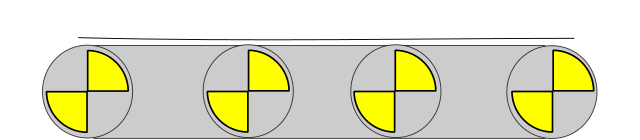
\includegraphics[width=0.7\linewidth]{obrazky/belt}
	\caption{Prepravný pás}
	\label{fig:belt}
\end{figure}
%%%%%%%%%%%%%%%%%%%%%%%%%%%%%%%%%
\begin{figure}[H]
	\centering
	\includegraphics[width=0.7\linewidth]{obrazky/trippleValve}
	\caption{Trojcestný ventil}
	\label{fig:trippleValve}
\end{figure}
%%%%%%%%%%%%%%%%%%%%%%%%%%%%%%%%%%%%%%%%%
\begin{figure}[H]
	\centering
	\includegraphics[width=0.7\linewidth]{obrazky/map}
	\caption{Mapa Slovenska}
	\label{fig:map}
\end{figure}
%%%%%%%%%%%%%%%%%%%%%%%%%%%%%%%%%%%%%%%%%%



%%%%%%%%%%%%%%%%%%%%%%%%%%%%%%%%%%%%%%%%%%%%
%%%%%%%%%%%%%%%%%%%%%%%
\begin{figure}[H]
	\centering
	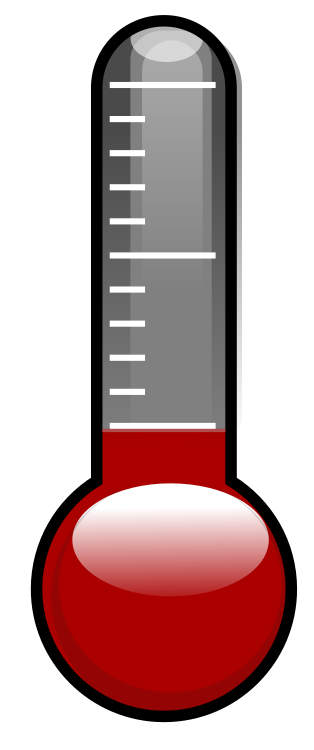
\includegraphics{obrazky/thermometer}
	\caption{Termometer}
	\label{fig:thermometer}
\end{figure}
\chapter{Integrácia grafického komponentu}

V tejto kapitole bližšie popíšem implementáciu prečerpávacej stanice. 

\section{Vytvorenie prečerpávacej stanice v Inkscape}

Nakreslenie jednotlivých častí komponentov prečerpávacej stanice v Inkscape bolo realizované pomocou ľavého bočného panela. Prečerpávacia stanica sa skladá z potrubí, indikátora úrovne hladiny vody, motora, a dvoch symbolov prítoku hladiny. Ako je možné vidieť na obrázku  \ref{picture1}.  


\begin{figure}[H]
	\begin{center}
		\includegraphics[width=0.6\linewidth] {obrazky/pump1.jpg}
		\caption{Grafické prostredie programu Inkscape s nakreslenou prečerpávacou stanicou}
		\label{picture1}
	\end{center}
\end{figure}


\section{Definovanie id v SVG}

Pre ovládanie JavaScriptom je nutné si pozrieť jednotlivé jedinečné identifikačné názvy. V .svg súboroch sú označované ako id. V zdrojovom kóde .svg súboru je to označené id="nazovElementu". Na ovládanie časti svg elementu v JavaScripte bude realizované cez CSS selektor, kde pristúpim k id svg cez značku \#.  Napríklad: paper.select("\#ventil"); .


\subsection{Object Properties}
Zistenie id je pomerne jednoduché v Inkscape. Klikneme pravým tlačidlom na daný komponent, ktorého id chceme vedieť, a potom na Objekt Properties.

Po kliknutí sa nám zobrazí okno s názvom Object Properties. 

\begin{figure}[H]
	\begin{center}
		\includegraphics [width=5cm]  {obrazky/obr3.png}
		\caption{Object Properties}
		\label{picture3}
	\end{center}
\end{figure}


Z obrázka č.\ref{picture3} možno vyčítať aké je ID, predvolené sú tam napríklad desc3072. Hodnoty je možné prepísať a zmeniť stlačením tlačidla Set. Pre nás je dôležitá hodnota v kolónke id - ventil. 

V okne Object Properties je možné nastaviť script na animovanie. Po kliknutí na Interactivity sa zobrazia ďalšie kolónky, kde je možné zadať akciu, ktorá má nastať.  


\subsection{XML Editor}
Ďalší spôsob získania informácii o svg cez Inkscape je cez zabudovaný XML Editor.
Stlačením klávesovej skratky SHIFT + CTRL + X alebo v hornej lište v menu vybrať ponuku Edit a na spodku je XML Editor. Následne sa zobrazí okno, ktoré je na obrázku \ref{xmlEditor}. XML Editor umožní zistiť ID jednotlivých komponentov, ale i hodnoty atribútov. 

\begin{figure}[H]
	\begin{center}
		\includegraphics[width=0.6\linewidth]  {obrazky/XmlEditor2.png}
		\caption{Xml Editor v Inkscape}
		\label{xmlEditor}
	\end{center}
\end{figure}



\section{Integrácia prečerpávacej stanice pre dynamické ovládanie SVG objektu}

Súborová štruktúra prečerpávacej stanice: 
\begin{itemize}
	\item index.html 
	\item PumpingStation.js
	\item PumpingStation.svg
	\item TestPumpingStation.js
\end{itemize}

\subsection{HTML súbor}
Do HTML súboru index.html pridáme párový tag $<$svg$>$.  Na toto miesto sa neskôr vykreslí SVG načítané zo súboru cez JavaScript. Môže sa tu uviesť i celý kód SVG obrázka. V prípade, že nebude v dokumente dané, kde presne sa nachádza SVG, tag tak sa pridá na najbližšie voľné miesto. 
\subsection{Kód}
\begin{lstlisting}
<svg 
	id="svgStanica" 
	viewBox="0 0 750 600" 
	width="100%" 
	height="100%"> 
</svg>
\end{lstlisting}

\subsection{Vysvetlenie kódu}
Atribúty v tagu sú prispôsobené na to, aby sa grafický element vykreslil responzívne na obrazovku.
\begin{itemize}
\item  \textbf{id} - jedinečný identifikátor. 
\item 	\textbf{viewBox} - je virtuálne okno, ktorým sa užívateľ uvidí svg obrázok. Je atribút, ktorý povoľuje špecifikovať danú množinu grafických komponentov, aby sa zobrazili v daných súradniciach x, y a šírke, výške. Hodnoty atribútov v viewBox sú štyri čísla - min-x, min-y, width a height. 
\item 	\textbf{width} a \textbf{height} je šírka a výška. Hodnoty atribútov je možné uviesť relatívne v percentách alebo absolútne v pixloch. 
\end{itemize}

Do HTML dokumentu sa pridajú jednotlivé JavaScriptové knižnice s ktoré bude daný grafický komponent používať. 
\begin{lstlisting}[language = HTML]
<script src="../js/snap.svg-min.js"></script>
<script src="PumpingStation.js"></script>
\end{lstlisting}

Musíme sa uistiť, aby sa načítali všetky JavaScriptové knižnice, pred spustením funkcií. To zabezpečíme pridaním  onload do tagu $<$body$>$. 
\begin{lstlisting}[language = HTML]
	<body onload="onPageLoad();">
\end{lstlisting}



\section{PumpingStation.js}
V súbore PumpingStation.js sú metódy na vizualizáciu grafického komponentu. V tejto časti je popis jednotlivých funkcií. 
Interface prečerpávacej stanice: 
\begin{itemize}
	\item onPageLoad();
	\item PumpingStation(nazovFileSVG, idDOMsvgElement);
    \item openValve1(isOpenValve1);
    \item animateTank(intPercent);
    \item rotateEngine(isRotating);
    \item openValve2(isOpenValve2);
    \item updateSchema01(isOpenValve1, intPercent, isRotating, isOpenValve2);
    \item updateSchema(updateData);
\end{itemize}

\subsection{onPageLoad()}
onPageLoad() sa spustí pri načítaní tela HTML súboru index.html. Následne spustí  PumpingStation(par1,, par2). Prvý parameter je udaný svg súbor vytvorení programom Inkscape. Druhý parameter je id tagu svg, kde sa vykreslí prečerpávacia stanica.

\begin{lstlisting}
function onPageLoad() {
	PumpingStation("PumpingStation.svg", "#svgStanica" );
}
\end{lstlisting}

\subsection{PumpingStation(par1, par2)}

Parametre pre PumpingStation sú názov svg súboru, a id, ktoré sa nachádza v tagu $<$svg$>$ html súbore.

Vo vnútri PumpingStation sa nachádza inicializácia globálnych atribútov. 
\begin{lstlisting}[language = HTML]
var paper;
var idValve, idValve1 idNadrz, idHladina, idEngineMotor;

function PumpingStation(nazovFileSVG, idDOMsvgElement) {
	paper = Snap(idDOMsvgElement);
	Snap.load(nazovFileSVG, function (f) {
		idHladina = "#hladina";
		idNadrz = "#nadrz";
		idValve = "#ventil";
		idValve2 = "#ventil2";
		idEngineMotor = "#engineMotor";
		paper.append(f);
	});
}
\end{lstlisting}

Atribút paper je globálna premenná cez ktorú sa bude pristupovať k metódam JavaScriptovej knižnice Snap.svg. Jej parameter je referencia na plochu, kde bude vykreslené SVG elementy.

Vo vnútri funkcie sa volá z Snap.svg API funkcia load(). Má parametre názov súboru, a funkciu, ktorú spustí následne po načítaní. 
Vo vnútri funkcie load() sa inicializujú globálne premenné.  
Premenné obsahujú CSS selektor id získaný z programu Inkscape. Premenné budú slúžiť ako parameter pri volaní funkcie paper.select(). Pre prípadné zmeny v id, sa dané id zmení na jednom mieste a nemusí sa prepisovať všade. 

Význam premenných je nasledový: 
\begin{itemize}
	\item idHladina - indikátor prítoku hladiny vody, 
	\item idNadrz - je miesto, kde bude prichádzať prítok vody,
	\item idValve1, idValve2 - je ventil, 
	\item idEngineMotor - je symbol rotora motora.
\end{itemize}

Načítaný .svg súbor sa zobrazí volaním metódy append. 

\subsection{animateTank(percento)}
V tejto metóde je zobrazená vizualizácia prítoku hladiny do nádrže. Ako parameter slúži percento vyplnenia. 

\begin{lstlisting}[language = HTML]
function animateTank(percento){
	var height = paper.select(idNadrz).getBBox().height;
	var y = paper.select(idNadrz).getBBox().y;
	var newHeight = height * (percento/100);
	var newY = y + height - newHeight;
	
	paper.select(idHladina).animate({
	y: newY,
	height: newHeight
	}, 1000);
}
\end{lstlisting}

Animovanie je realizované cez metódu animate zo Snap.svg API. 
Význam lokálnych premenných: 
\begin{itemize}
	\item height - výška nádrže do, ktorej bude pritekať voda,  získaná volaním metódy getBBox(),
	\item y - súradnica y - navýšením, alebo znížením hladiny sa mení súradnica y, a x zostava nezmenená,
	\item newHeight - vypočítaná nová výška hladiny podľa daného percenta, 
	\item newY - je vypočítaná súradnica - osi y. 
\end{itemize}

Volaním metódy animate, sa zanimuje daný element, v tomto prípade to bude hladina nádrže. Metóda má nasledovné parametre: \begin{itemize}
	\item atribúty - v pároch udané atribúty, ktoré sa zmenia. Zmení sa iba výška a os y, ostatné atribúty zostávajú nezmenené.
	\item rýchlosť animácie udaná v milisekundách. 
\end{itemize}

 
\subsection{openValve1(isOpen)}
Indikátor prítoku hladiny do prečerpávacej stanice je ventil, ktorý mení farbu. Ak je nastavený parameter isOpen na true, tak farba ventila bude zelená, v inom prípade červená. 
Zmena farby je realizovaná volaním metódy attr zo Snap.svg API, ktorá nastavila atribút fill daného elementu na danú farbu. Farba zmeny je zapísaná termálnym operátorom. 
Pre zmenu farby v druhom elemente je zápis identický až na to, že je zmena pri volaní select - na idValve2. 
\begin{lstlisting}
function openValve1(isOpen){
	paper.select(idValve).attr({
	fill: ((isOpen === "true") ?   "green" : "red")
	});
}
\end{lstlisting}



\subsection{rotateEngine(isRotating)}
Táto metóda bude rotovať až dovtedy pokým sa nezmení parameter isPaused. Rotácia motora je zabezpečená vnorenou metódou rotateLeft. Tá sa volá v toggleRotation(), kde v má parameter element vrtuliek čerpadla. 

Popis metódy rotateLeft():
\begin{itemize}
\item animationRunning - nastavené na true, znamená to, že animácia ešte beží
\item stringT0 - je transformačný string - potrebný na rotáciu vrtuliek čerpadla. Uhol rotácie je nulový, a súradnice stredovej osi x, y sú získané volaním metódy elementu getBBox().cx a getBBox().cy. 
\item transform() - je metóda z Snap.svg knižnice, ktorá umožní nastaviť transformáciu rotácie, kde parametrom je transformančný string. 
\item if(!(isPaused)){..} - je podiemka, ktorá zaručí opakované rotovanie elementu. 
\item stringT360 - je transformačný string, ktorý zrotuje element o uhol 360 stupňov zo stredom súradnicovej osi elementu. 
\item animate() - je metóda, kde animujem transformáciu z uhlu 0 stupňov na 360 stupňov. Ako parametre sú:
\subitem - párový atribút transform s hodnotou transformačného stringu, 
\subitem - rýchlosť animácie v milisekundách - 2000 ms, 
\subitem - mina objekt, ktorý zaručí lineárny plynulý pohyb, 
\subitem - callback funkcia, ktorá sa spustí po dokončení animácie. Toto zabezpečí opakované spustenie animácie rotácie elementu. 
\item else - ak skončí animácia - tak sa nastaví animationRunning na hodnotu false. 
\end{itemize}

\subsubsection{Kód metódy} 
\begin{lstlisting}
var isPaused = true;
var animationRunning = false;
function rotateEngine(isRotating){
	isPaused = isRotating;

	function toggleRotation() {
		if (!animationRunning && isPaused) {
			isPaused = false;
			rotateLeft(paper.select(idEngineMotor));
		} else {
			isPaused = true;}
	}
	toggleRotation();

	function rotateLeft(element) {
		animationRunning = true;
		var stringT0 = "R0,"+ element.getBBox().cx 	+ ","+
		element.getBBox().cy;
		element.transform(stringT0);

	if (!(isPaused)) {
		var stringT360 = "R360,"+ element.getBBox().cx 	+ ","+
		element.getBBox().cy;
		element.animate({
		 transform: stringT360 },
		 2000, 
		 mina.linear, 
		 rotateLeft.bind(null, element));
		} else { animationRunning = false;}
	}
}
\end{lstlisting}


\section{updateSchema()}

Metóda updateSchema01 zabezpečí aktualizáciu grafického komponentu. Parametre má nasledovné: 
\begin{itemize}
\item isOpenValve - boolean hodnota, ktorá nastaví indikátor prítoku vody, v prípade true - na zelený, v opačnom na červený. 
\item intPercento - je integer hodnota v rozsahu od 0-100. Vyjadruje percentuálne naplnenie nádrže. 
\item isRotating - boolean hodnota, ktorá nastaví otáčanie motora, až pokým sa znova nezavolá. 
\item isOpenValve - boolean hodnota druhého ventila. 
	
\end{itemize}

\begin{lstlisting}
function updateSchema01(isOpenValve1, intPercent, isRotating, isOpenValve2) {
	openValve1(isOpenValve1) ;
	animateTank(intPercent);
	rotateEngine(isRotating);
	openValve2(isOpenValve2);
}
\end{lstlisting}

Dáta vyjadrené vo formáte \ac*{JSON}. Zároveň je to interfejsná metóda k grafickému komponentu Pumping Station. Toto je príklad objektu update dátami na nastavenie hladiny nádrže na 20 percent a s ventilami, a rotorom zapnutým.  
\begin{lstlisting}
var updateData = {
	"valve1": "true",
	"tank": "20",
	"engineRotation": "true",
	"valve2": "true"
};
\end{lstlisting}
Metóda updateSchema s parametrom objekt updateData, aktualizuje grafický komponent na dané hodnoty. Zároveň je  to interfejsná metóda k REST API prečerpávacej stanice. Na obrázku \ref{fig:updateSchema} je zobrazený animovaný komponent s vopred pripravenými dátami. 
\begin{lstlisting}
function updateSchema(updateData){
	updateSchema01(updateData.valve1, updateData.tank, updateData.engineRotation, updateData.valve2);
}
\end{lstlisting}


\begin{figure}[H]
\centering
\includegraphics[width=0.7\linewidth]{obrazky/updateSchema}
\caption{Prečerpávacia stanica po vykonaní príkazu updateSchema(updateSchema);}
\label{fig:updateSchema}
\end{figure}
\chapter{REST API}

\section{REST API pre grafické komponenty}
Grafické komponenty pre vizualizáciu dát zo systému D2000 budú umiestňované na HTML stránkach použitých ako súčasť web rozhrania frameworku D2000 WebSuite.

Tento framework je založený na technológii Java Enterprise Edition a Java Server Faces.

Životný cyklus webovej stránky - načítanie stránky s technologickou schémou, pre prvé zobrazenie kompletnej schémy je potrebný plný dáta set.


Príklad REST URL:\\
\url{http://localhost:8080/scada-demo/rest/pumpingstation/gatfulldataset}


Príklad JSON dát z grafického komponentu prečerpávacia stanica: 
\begin{lstlisting}
var updateData = {
	"valve1": "false",
	"tank": "0",
	"engineRotation": "false",
	"valve2": "false"
};
\end{lstlisting}


Zobrazenie stránky v rámci jednej http session, typicky vo web aplikáciách kde sa užívateľ prihlási pomocou mena a hesla, trvanie jeho session je obmedzené na predom stanovený čas, napríklad jednu hodinu.


Pri zobrazení zložitejšej technologickej schémy, je potrebné optimalizovať množstvo prenesených dát a interakciu z DOM stránky. Preto je počas zobrazenia schémy výhodne implementovať čiastočne aktualizácie, ktoré menia len dotknuté časti schémy a nie celú schému ako je tomu pri načítaní stránky.  

Príklad REST URL:\\ ň
\url{http://localhost:8080/scada-demo/rest/pumpingstation/getvalvestatus}
príklad JSON dát:
\begin{lstlisting}
var updateDataTank = {"tank": "86"};
\end{lstlisting}}

príklad REST URL\\ \url{http://localhost:8080/scada-demo/rest/pumpingstation/getrotorstatus}
príklad JSON dát: (môžeš uviesť dáta z puding stati on)
príklad REST URL\\ \url{http://localhost:8080/scada-demo/rest/pumpingstation/getwaterlevel}
príklad JSON dát: (môžeš uviesť dáta z puding stati on)


\section{Data binding pre system D2000}
Priama väzba v prípade jednoduchých schém. Jednoduchá schéma predstavuje vizualizáciu meraného alebo počítaného bodu v systéme D2000. Takáto vizualizácia je realizovaná pomocou widgetu jedna sa o mapovanie 1:1.
%(môžeš uviesť príklad ako teplomer alebo ručičkový merač, obrázky) 
Zložitejšie schémy pozostávajúce z vizualizácie výrobného procesu alebo komplexnej technológie sú mapované vo vzťahu n:1, teda jedna schéma vizualizuje dáta z n meraných alebo počítaných bodov, pripadne získava dáta cez asynchrónne volania RPC (remote procedure call) systému D2000.

Ak to vyžaduje logika aplikácie, server implementuje dátový zdroj (service), ktorý agreguje dáta a systémové udalosti. Pre dosiahnutie real-time odozvy web rozhrania výhodne použiť obojstrannú komunikáciu medzi web browserom a serverom - technológiu web sockets.

% (môžeš uviesť niečo o web socketoch, skús pohľadať na webe), vo stvrtok to mozme doladit.

\chapter{Analýza výkonnosti a obmedzení }
Pre meranie výkonnosti vizualizácie grafických komponentov v reálnom čase zadefinujem v nasledujúce kritéria
\begin{itemize}
	\item počet komponentov, 
	\item čas načítania stránky, 
	\item čas vykonania zmeny atribútov v komponentoch.
\end{itemize}

Testy boli vykonané vo webovom prehliadači Chrome verzia 45 a Firefox verzia 40.  

V teste boli použité nasledujúce navrhnuté komponenty:
\begin{itemize}
	\item teplomer, 
	\item prečerpávacia stanica, 
	\item trojcestný ventil, 
	\item mapa Slovenska, 
	\item prepravný pás. 
\end{itemize}

Objekty boli v rovnakom zastúpení v jednom HTML súbore  v počtoch: 1,5,10,25, 50, 100.
Ukážka testovacej situácie je na obrázku TODO SCREEN. 
A výsledky sú uvedené v tabuľke TODO TABULKA. 


\newpage
Alebo vytvorim test -
http://jsperf.com/
- kde porovnam SVG smil animaciu s snap.svg.js
ktore je v kapitole 4 - strana vtedy bola 20

%
%\url{http://www.sitepoint.com/advanced-snap-svg/}
%Performance Improvements
%
%One way to improve performance when manipulating the DOM is using DocumentFragments. Fragments are minimal containers for DOM nodes. Introduced a few years ago, they allow you to inexpensively manipulate entire subtrees, and then clone and add a whole subtree with n nodes to our page with 2 method calls instead of n. The actual difference is explained in details on John Resig’s blog.
%
%Snap allows for native use of fragments as well, with two methods:
%
%Snap.parse(svg) takes a single argument, a string with SVG code, parses it and returns a fragment that can be later appended to any drawing surface.
%
%Snap.fragment(varargs) takes a variable number of elements or strings, and creates a single fragment containing all the elements provided.
%
%Especially for large svg drawings, fragments can lead to a huge performance saving, when used appropriately.
%
%
%\newpage
%
%%http://www.html5rocks.com/en/tutorials/speed/high-performance-animations/
%
%\url{http://caniuse.com/#feat=svg-html}
%
%
%***********************
%
%Animácia pozície 
%- transform: translate(npx, npy);
%
%Animácia škály 
%- transform: scale(n);
%
%Animácia otáčania
%- transform: rotate(ndeg)
%
%Animácia neprehľadnosti 
%- opacity: 0..1;
%
%*************************
%
%%\url{http://www.svgopen.org/2008/papers/74-HighPerformance_GML_to_SVG_Transformation_for_the_Visual_Presentation_of_Geographic_Data_in_WebBased_Mapping_Systems/}
%
%
%\textbf{Transformation}
%\textit{scale}(sx, sy) - zmenim veľkosť tvaru na danane suradnice, 
%\textit{translate}(tx, ty) - presuniem na ine miesto - zmenim suradnice 
%
%%\url{https://developers.google.com/web/fundamentals/performance/rendering/optimize-javascript-execution?hl=en}
%
%Podpora svg v prehliadačoch
%\url{http://caniuse.com/#feat=svg}
%
%\url{http://www.schepers.cc/svg/blendups/embedding.html}
\chapter{Vzorová sada}

Vzorová sada grafických komponentov SCADA systémov obsahuje:
\begin{itemize}
	\item Thermometer,
	\item Triple Valve, 
	\item Map of Slovakia,
	\item Pumping station, 
	\item Conveyor belt 
	
\end{itemize}

\begin{figure}[H]
\centering
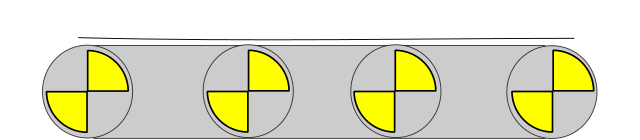
\includegraphics[width=0.7\linewidth]{obrazky/belt}
\caption{}
\label{fig:belt}
\end{figure}


\begin{figure}[H]
	\centering
	\includegraphics[width=0.7\linewidth]{obrazky/map}
\caption{}
\label{fig:map}
\end{figure}
\begin{figure}[H]
	\centering
	\includegraphics[width=0.7\linewidth]{obrazky/pump}
\caption{}
\label{fig:pump}
\end{figure}
\begin{figure}[H]
	\centering
	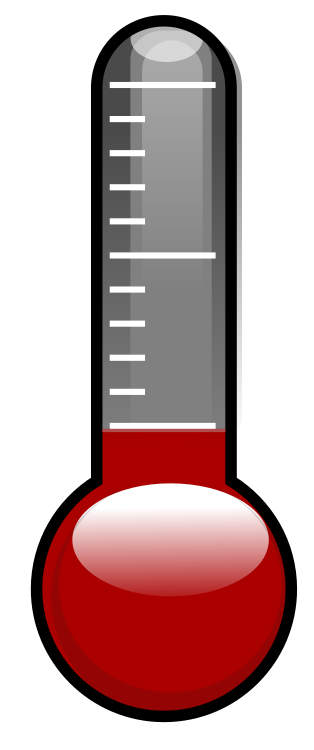
\includegraphics{obrazky/thermometer}
\caption{}
\label{fig:thermometer}
\end{figure}

\begin{figure}[H]
\centering
\includegraphics[width=0.7\linewidth]{obrazky/trippleValve}
\caption{}
\label{fig:trippleValve}
\end{figure}

\chapter*{Záver}

Cieľom práce bolo navrhnúť riešenie pre vizualizáciu SCADA komponentov vo webovom prehliadači. Mojou úlohou v záverečnej práci bolo vytvoriť univerzálny postup pre animáciu komponentov. 

Doterajšie riešenie nevyužívalo všetky možnosti štandardu HTML5 a SVG, hlavne animácie a transformácie. Navrhnuté riešenie použitím kombinácie SVG a JavaScriptovej knižnice je vhodné a užitočné pre vizualizáciu SCADA systémov. Navrhnuté riešenie vhodnejšie využíva zdroje na strane webových klientov čo umožňuje nasadenie na menej výkonných zariadeniach. 



Úspešne som vytvorila postup vizualizácie a vzorovú sadu grafických komponentov,na ktorých som si vyskúšala vizualizovanie. 
Grafický komponent som v .svg formáte nakreslila cez Inkscape. Pomocou knižnice Snap.svg som pridávala funkcie na animovanie a manipulovanie grafického komponentu. Navrhla som jednoduchý REST API interface, ktorý komunikuje so SCADA systémom. 

Výsledná sada je vhodná pre platformy ako napríklad tablety, mobilné telefóny a iné. 
Všetky zdrojové kódy práce sú v Git repository na GitHube\cite{github}, kde je odkaz aj na webovú stránku, kde je implementovaná vzorová sada..  Moje riešenie používa knižnicu a softvér, ktorý sú open-source.







%%%%%%%%%%%%%%%%%%%%%%%%%%%%%%%%%%%%%%%%%%%%%%%%%%%%%%%%%%%%%%%%%%%%%%%%%%%%%
\begin{thebibliography}{99}                                \label{literatura}
%\addcontentsline{toc}{section}{Literatúra}
\addcontentsline{toc}{chapter}{Zoznam použitej literatúry}




\bibitem{Dawber}
Dawber D.,
{\it Learning Raphael JS Vector Graphics }, 
 Packt Publishing, 2013, ISBN 978-1-78216-916-1
         
 
 
\bibitem{Wilson} Wilson CH., {\it RaphaelJs Graphic and visualization on the web} , 
O'Reilly Media, 2013, ISBN 978-1-449-36536-3
         

\bibitem{Haverbeke}
Haverbeke M., 
{\it Eloquent Javascript} 2. vyd. No Starch Press, 2014, ISBN 978-1-59327-584-6


\bibitem{Zakas}
Zakas N. Z., 
{\it JavaScript pro webové vývojáře Programujeme profesionálně},
 v1. vyd. Brno:Computer Press, a.s., 2009,  ISBN 978-80-251-2509-0

\bibitem{Suehring}
Suehring S., 
{\it JavaScript krok za krokem},
1. vyd. Brno:Computer Press, 2008, ISBN 978-80-251-2241-9

\bibitem{ZakasA}
Zakas N. C., McPeak J., Fawcett J.,
{\it Profesionálně Ajax},
Zoner Press, 2007,  ISBN 978-80-86815-77-0

\bibitem{Eisenberg}
Eisenberg D. J., {\it SVG Essentials}, 
O'Reilly Media 2002, ISBN  978-0-596-00223-7,  dostupné na \url{http://commons.oreilly.com/wiki/index.php/SVG_Essentials}

\bibitem{Richardson}
Richardson L., Amundsen M., {\it RESTful Web APIs} 
1. vyd. O'Reilly Media, 2013, 
ISBN 978-1-449-35806-8

\bibitem{Allamaraju}
Allamaraju S., {\it RESTful Web Services Cookbook} 
1. vyd. O'Reilly Media, 2010, 
ISBN 978-0-596-80168-7

\bibitem{snapsvg}
The JavaScript SVG library for the modern web,
\url{http://snapsvg.io/}.


\bibitem{Raphael}
\url{ http://raphaeljs.com/}

\bibitem {d3js}
\url {http://d3js.org/}

\bibitem{snapsvg}
 \url{http://snapsvg.io/}
 
 \bibitem{svgjs}
 \url{http://www.svgjs.com/}


\bibitem {Inkscape}
Inkscape is a professional vector graphics editor for Windows, Mac OS X and Linux. It's free and open source.
\url {http://www.inkscape.org/en/about/features/}

\end{thebibliography}	%  Literatura
%%%%% \MakeBibliography 

\chapter*{Zoznam skratiek}
\begin{acronym}
\acro{API}{Application Programming Interface}
\acro{CSS}{Cascading Style Sheets}
\acro{D3}{Data Driven Document}
\acro{DOM}{Document Object Model}
\acro{DPI}{Dots Per Inch}
\acro{GIF}{Graphics Interchange Format}
\acro{HTML}{Hyper Text Markup Language} 
\acro{JPEG}{Join Photographic Experts Group} 
\acro{JSON}{JavaScript Object Notation}
\acro{PPI}{Pixels Per Inch}
\acro{REST}{Representational State Transfer}
\acro{RGB}{Red Green Blue}
\acro{RPC}{Remote Procedure Call}
\acro{SCADA}{Supervisory Control and Data Acquisition} 
\acro{SMIL}{Synchronized Multimedia Integration Language}
\acro{SVG}{Scalable Vector Graphics} 
\acro{VML}{Vector Markup Language}
\acro{W3C}{World Wide Web Consortium}
\acro{WYSIWYG}{What You See Is What You Get}
\acro{XML}{EXtensible Markup Language}
\acro{MES} {Manufacturing Execution System}
\acro{RAD} {Rapid Application Development}
 
\end{acronym}

%pridat typy licencie.. 



\appendix
\chapter{UML diagramy}
	\section{Usecase diagram použitia SCADA systémov}
	\begin{figure}[H]
		\centering
		\includegraphics[width=0.50\linewidth]{uml/usecase.png}
		\caption{Usecase diagram použitia SCADA systémov}
		\label{fig:USECASE}
	\end{figure}

	\section{Postup načítania SVG súboru v HTML}
\begin{figure}[H]
	\centering
	\includegraphics[width=0.70\linewidth]{uml/aktivityInicializacie}
	\caption{Postup načítania SVG súboru v HTML dokumente}
	\label{fig:aktivity1}
\end{figure}

\section{Postup zistenia id elementu}

\begin{figure}[H]
	\centering
	\includegraphics[width=0.6\linewidth]{uml/aktivity2.png}
	\caption{Postup zistenia id elementu a jeho aktualizovanie}
	\label{fig:ovladanie}
\end{figure}







\section{Diagram tried vzorovej sady}
Diagram tried vzorovej sady je na obrázku \ref{fig:classD} . 
\begin{figure}[hp]
	\centering
	\includegraphics[width=0.9\linewidth]{uml/classDiagramTried}
	\caption{Diagram tried vzorovej sady grafických komponetov}
	\label{fig:classD}
\end{figure}





\end{document}